\chapter{Experimental Results}
\label{chap:experiment}
In this Chapter we evaluate our method on three real-world surveillance video benchmark datasets and analyze the experimental results in detail. Furthermore, we will compare our model with others popular approaches.

\begin{figure}[!htbp]
	\renewcommand{\thesubfigure}{\arabic{subfigure}}
	%\renewcommand{\thefigure}{\arabic{figure}}
	\makeatletter
	\renewcommand{\@thesubfigure}{(\thesubfigure)\space}
	\renewcommand{\p@subfigure}{\thefigure.}
	\makeatother
	\centering
	\subfigure[16.6\%]{
		\label{fig:subfigure:1}
		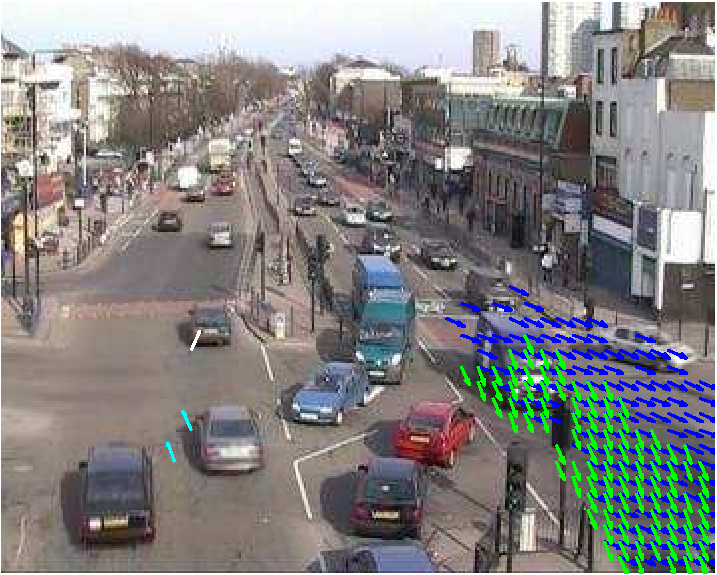
\includegraphics[width=3.7cm, height=2.5cm]{figures/qmul/t1-crop.pdf}}
	\subfigure[15.9\%]{
		\label{fig:subfigure:2}
		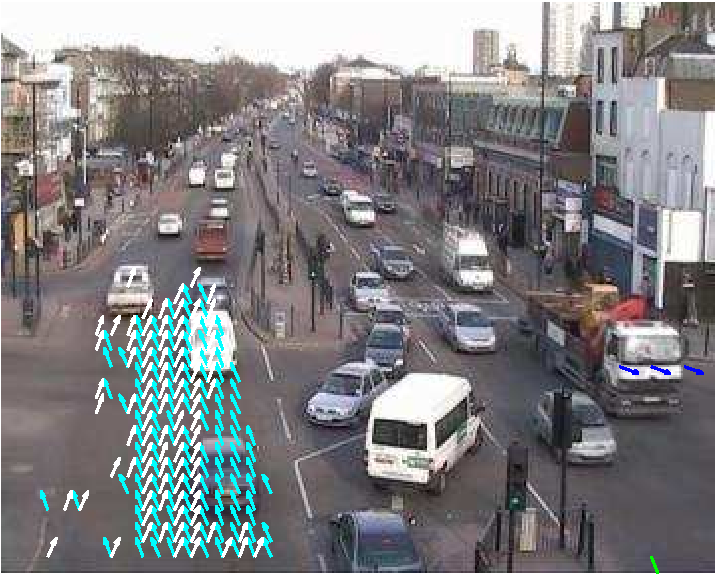
\includegraphics[width=3.7cm, height=2.5cm]{figures/qmul/t2-crop.pdf}}
	\subfigure[15.8\%]{
		\label{fig:subfigure:3}
		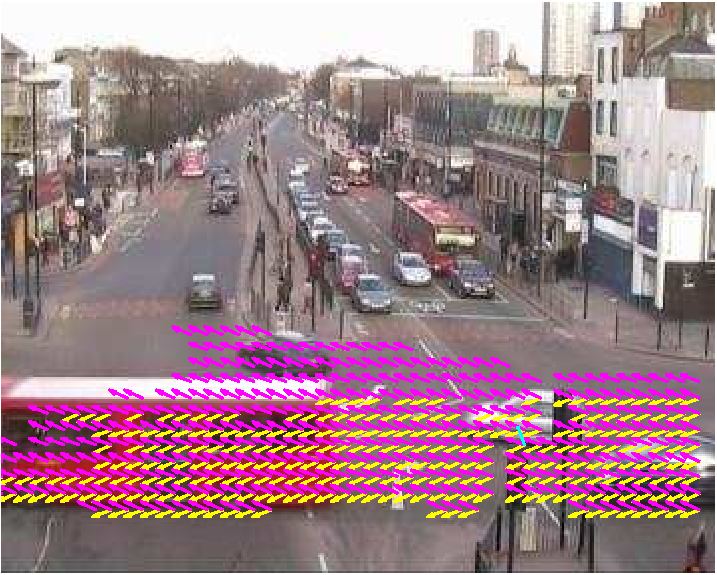
\includegraphics[width=3.7cm, height=2.5cm]{figures/qmul/t3-crop.pdf}}
	\subfigure[9.8\%]{
		\label{fig:subfigure:4}
		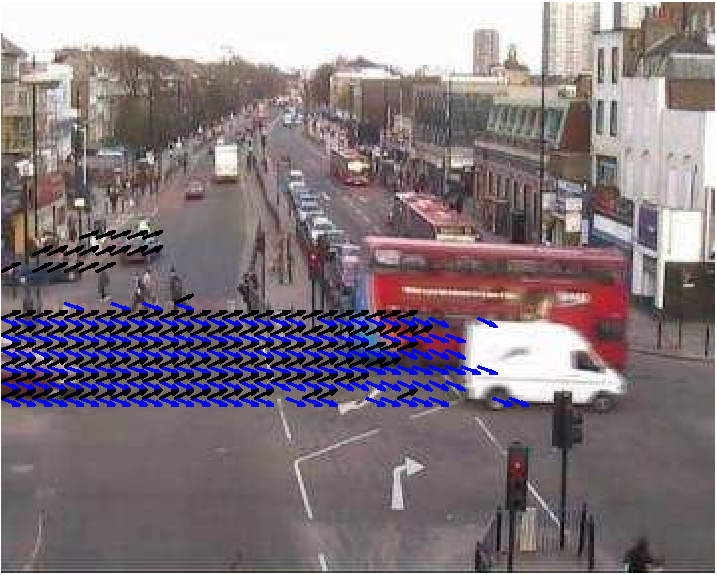
\includegraphics[width=3.7cm, height=2.5cm]{figures/qmul/t4-crop.pdf}}
	\subfigure[6.2\%]{
		\label{fig:subfigure:5}
		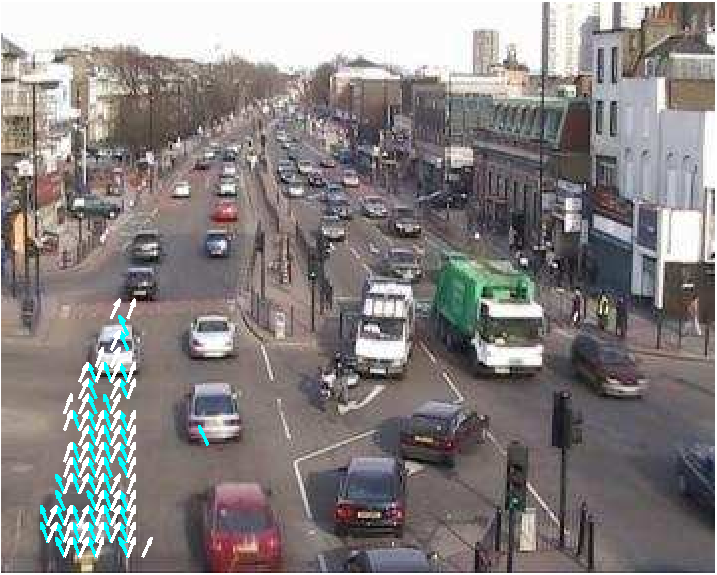
\includegraphics[width=3.7cm, height=2.5cm]{figures/qmul/t5-crop.pdf}}
	\subfigure[5.7\%]{
		\label{fig:subfigure:6}
		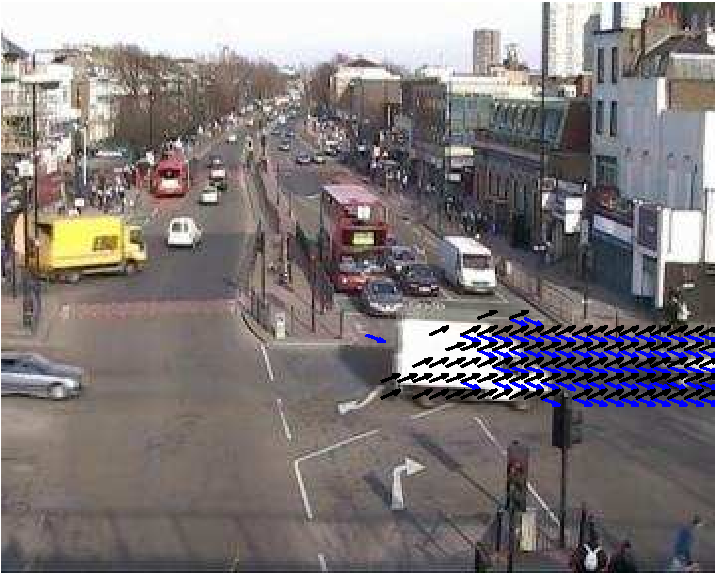
\includegraphics[width=3.7cm, height=2.5cm]{figures/qmul/t6-crop.pdf}}
	\subfigure[3.5\%]{
		\label{fig:subfigure:7}
		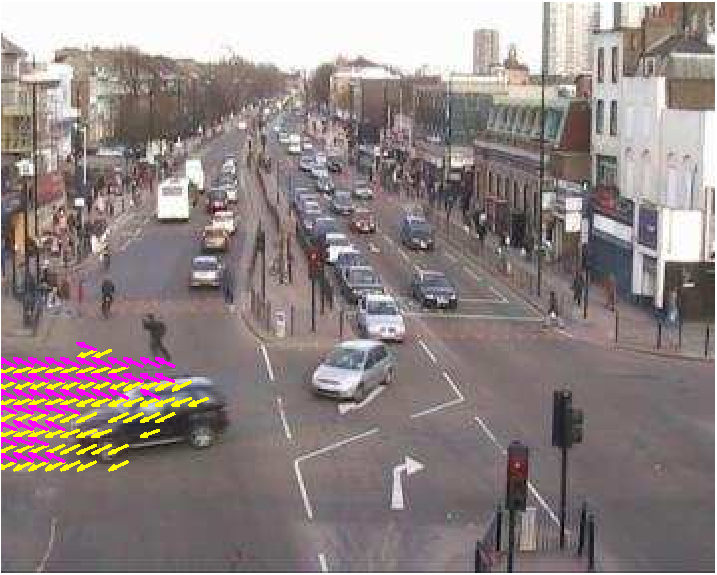
\includegraphics[width=3.7cm, height=2.5cm]{figures/qmul/t7-crop.pdf}}
	\subfigure[3\%]{
		\label{fig:subfigure:8}
		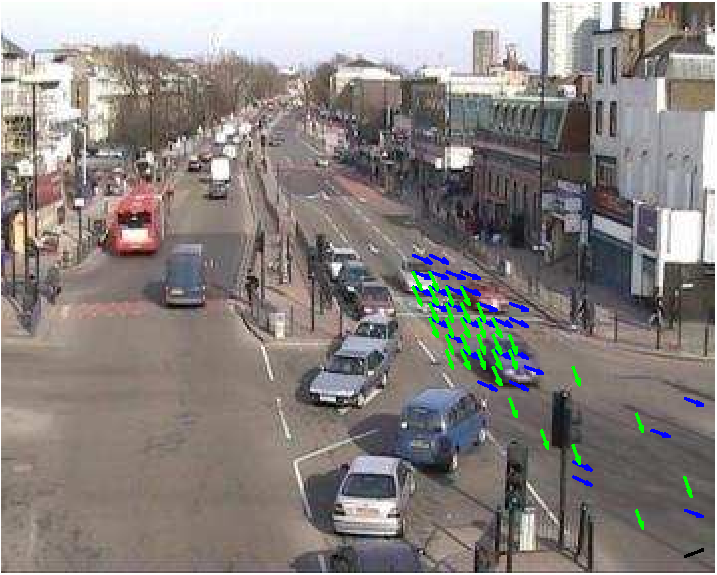
\includegraphics[width=3.7cm, height=2.5cm]{figures/qmul/t8-crop.pdf}}
	\subfigure[2.7\%]{
		\label{fig:subfigure:9}
		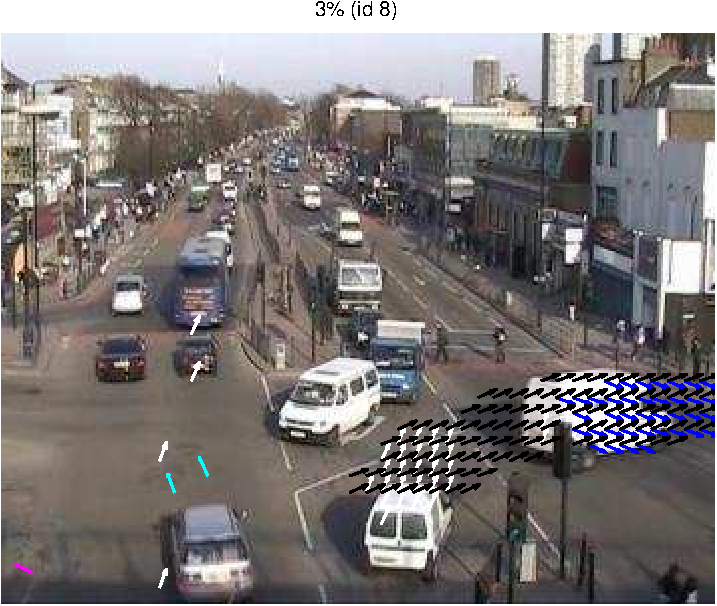
\includegraphics[width=3.7cm, height=2.5cm]{figures/qmul/t9-crop.pdf}}
	\subfigure[2.7\%]{
		\label{fig:subfigure:10}
		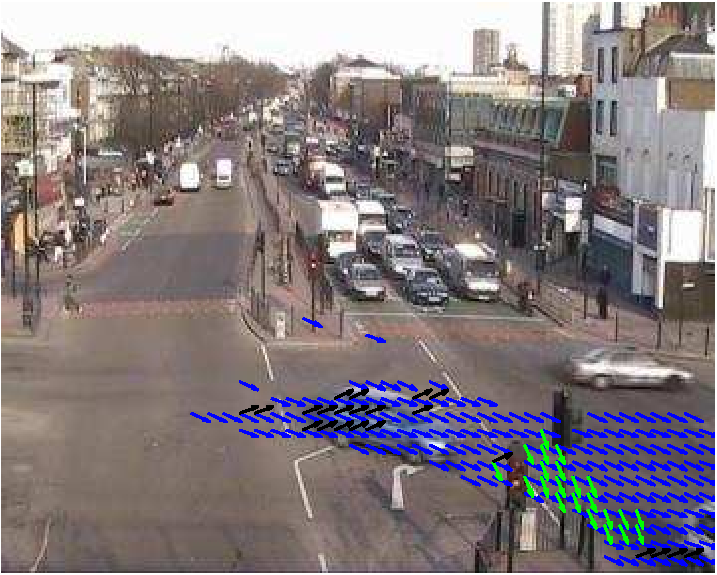
\includegraphics[width=3.7cm, height=2.5cm]{figures/qmul/t10-crop.pdf}}
	\subfigure[2.5\%]{
		\label{fig:subfigure:11}
		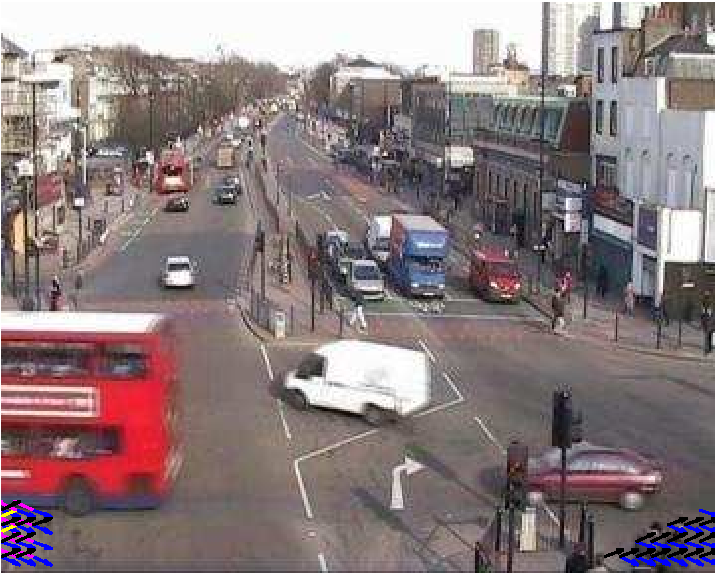
\includegraphics[width=3.7cm, height=2.5cm]{figures/qmul/t11-crop.pdf}}
	\subfigure[1.9\%]{
		\label{fig:subfigure:12}
		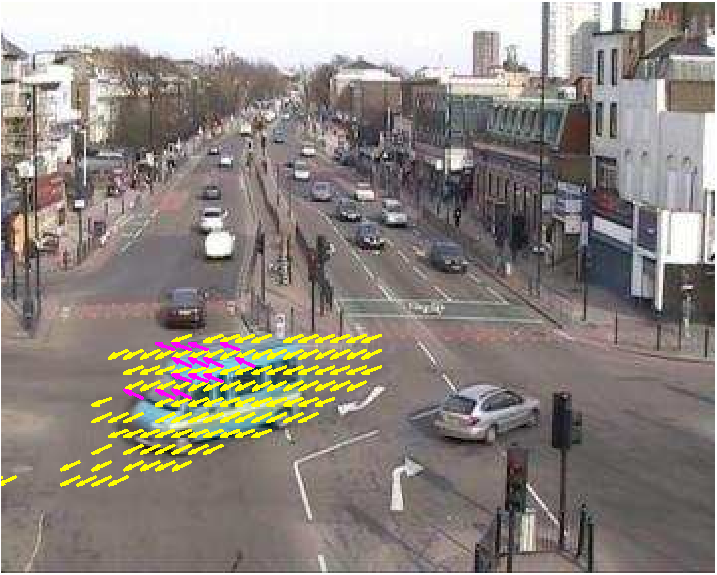
\includegraphics[width=3.7cm, height=2.5cm]{figures/qmul/t12-crop.pdf}}
	\subfigure[1.8\%]{
		\label{fig:subfigure:13}
		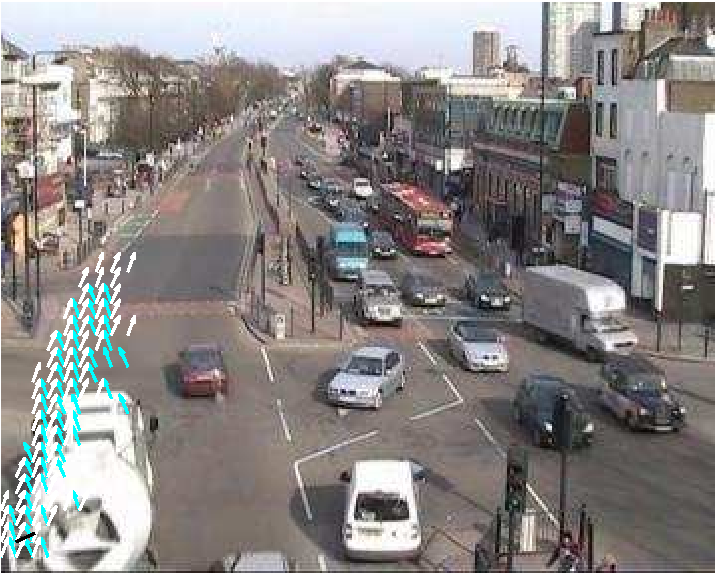
\includegraphics[width=3.7cm, height=2.5cm]{figures/qmul/t13-crop.pdf}}
	\subfigure[1.7\%]{
		\label{fig:subfigure:14}
		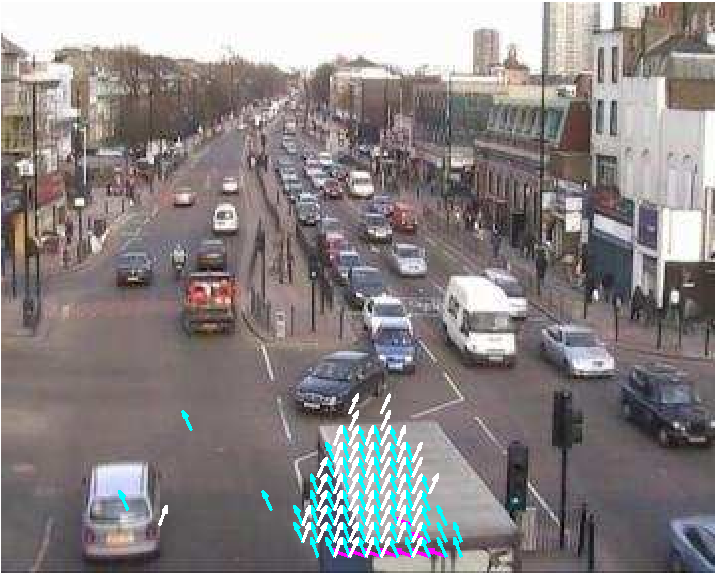
\includegraphics[width=3.7cm, height=2.5cm]{figures/qmul/t14-crop.pdf}}
	\subfigure[1.7\%]{
		\label{fig:subfigure:15}
		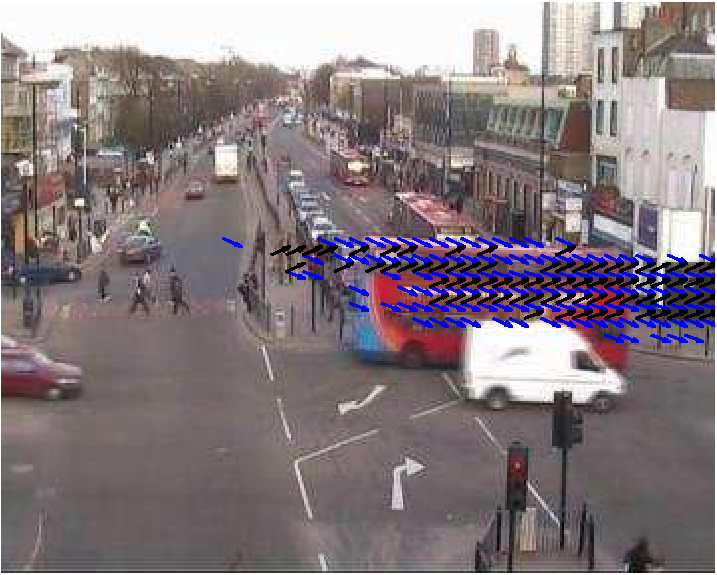
\includegraphics[width=3.7cm, height=2.5cm]{figures/qmul/t15-crop.pdf}}
	\subfigure[1.6\%]{
		\label{fig:subfigure:16}
		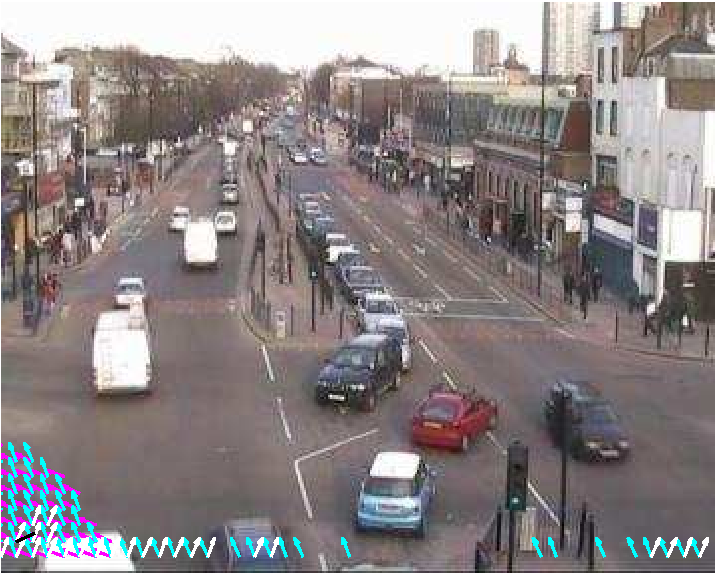
\includegraphics[width=3.7cm, height=2.5cm]{figures/qmul/t16-crop.pdf}}
	\subfigure[1.5\%]{
		\label{fig:subfigure:17}
		
		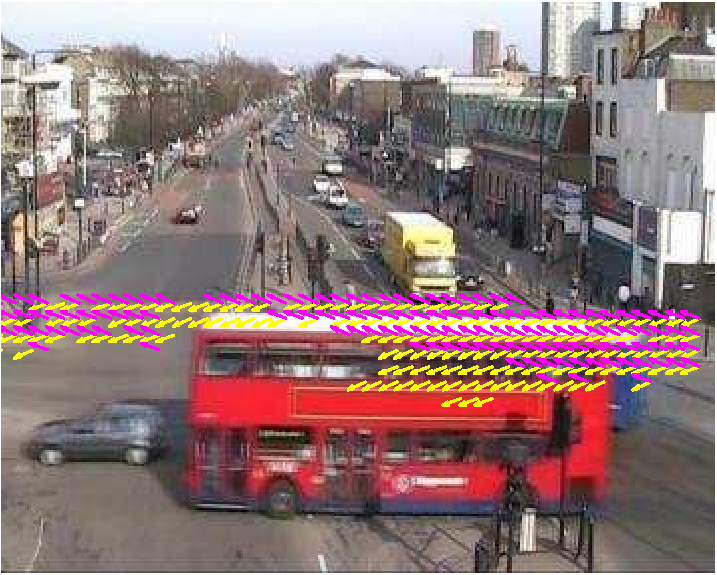
\includegraphics[width=3.7cm, height=2.5cm]{figures/qmul/t17-crop.pdf}}
	\subfigure[1.2\%]{
		\label{fig:subfigure:18}
		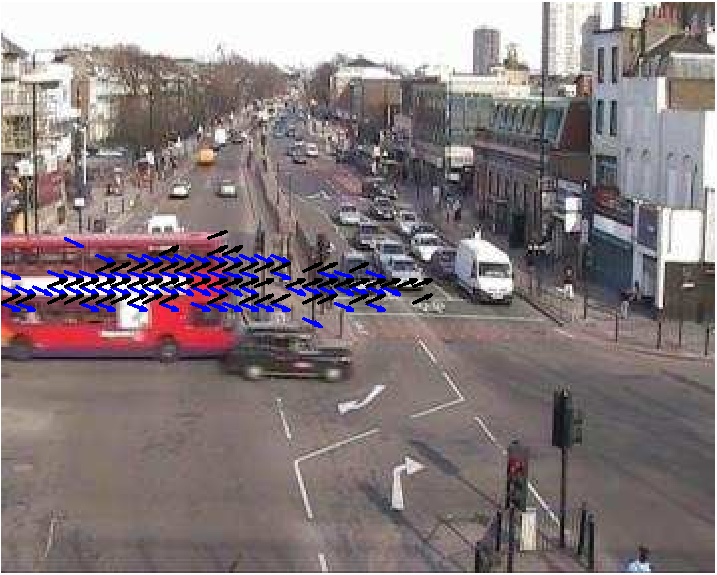
\includegraphics[width=3.7cm, height=2.5cm]{figures/qmul/t18-crop.pdf}}
	\subfigure[1\%]{
		\label{fig:subfigure:19}
		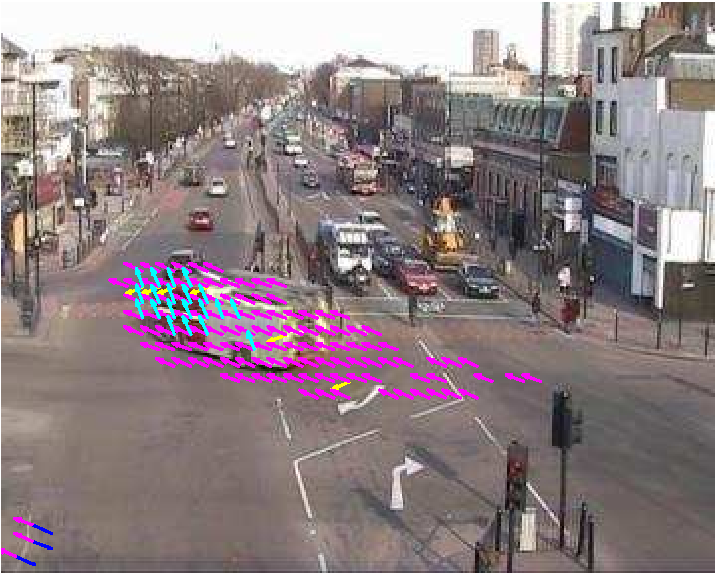
\includegraphics[width=3.7cm, height=2.5cm]{figures/qmul/t19-crop.pdf}}
	\subfigure[1\%]{
		\label{fig:subfigure:20}
		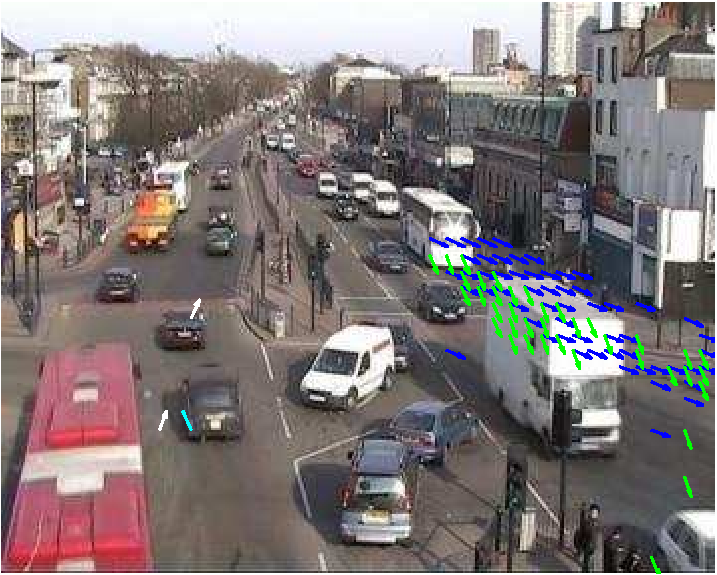
\includegraphics[width=3.7cm, height=2.5cm]{figures/qmul/t20-crop.pdf}}
	\subfigure[0.9\%]{
		\label{fig:subfigure:21}
		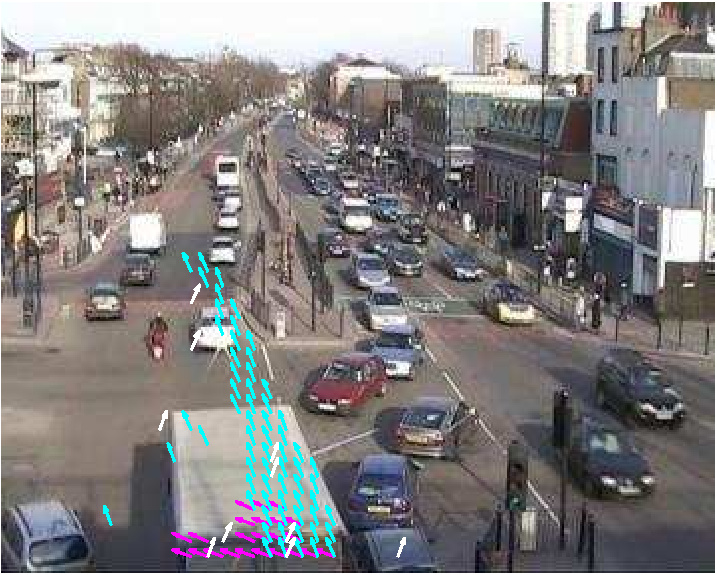
\includegraphics[width=3.7cm, height=2.5cm]{figures/qmul/t21-crop.pdf}}
	\subfigure[0.8\%]{
		\label{fig:subfigure:22}
		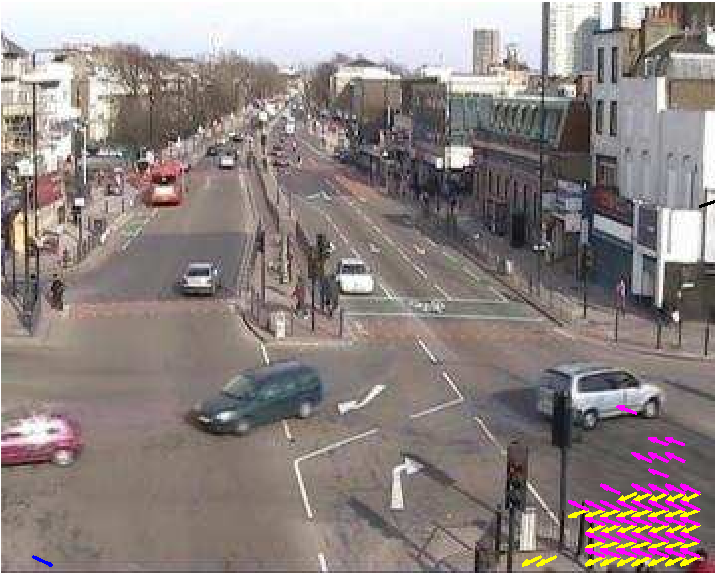
\includegraphics[width=3.7cm, height=2.5cm]{figures/qmul/t22-crop.pdf}}
	\subfigure[all possible lanes]{
		\label{fig:subfigure:qmul_path}
		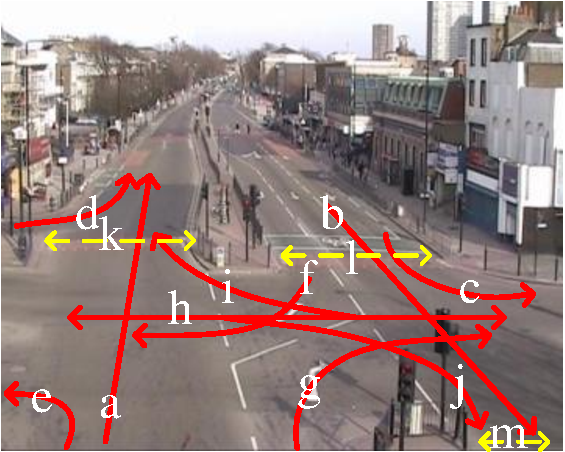
\includegraphics[width=3.7cm, height=2.5cm]{figures/qmul/qmul_path-crop.pdf}}
	\subfigure[colors for directions]{
		\label{fig:directions}
		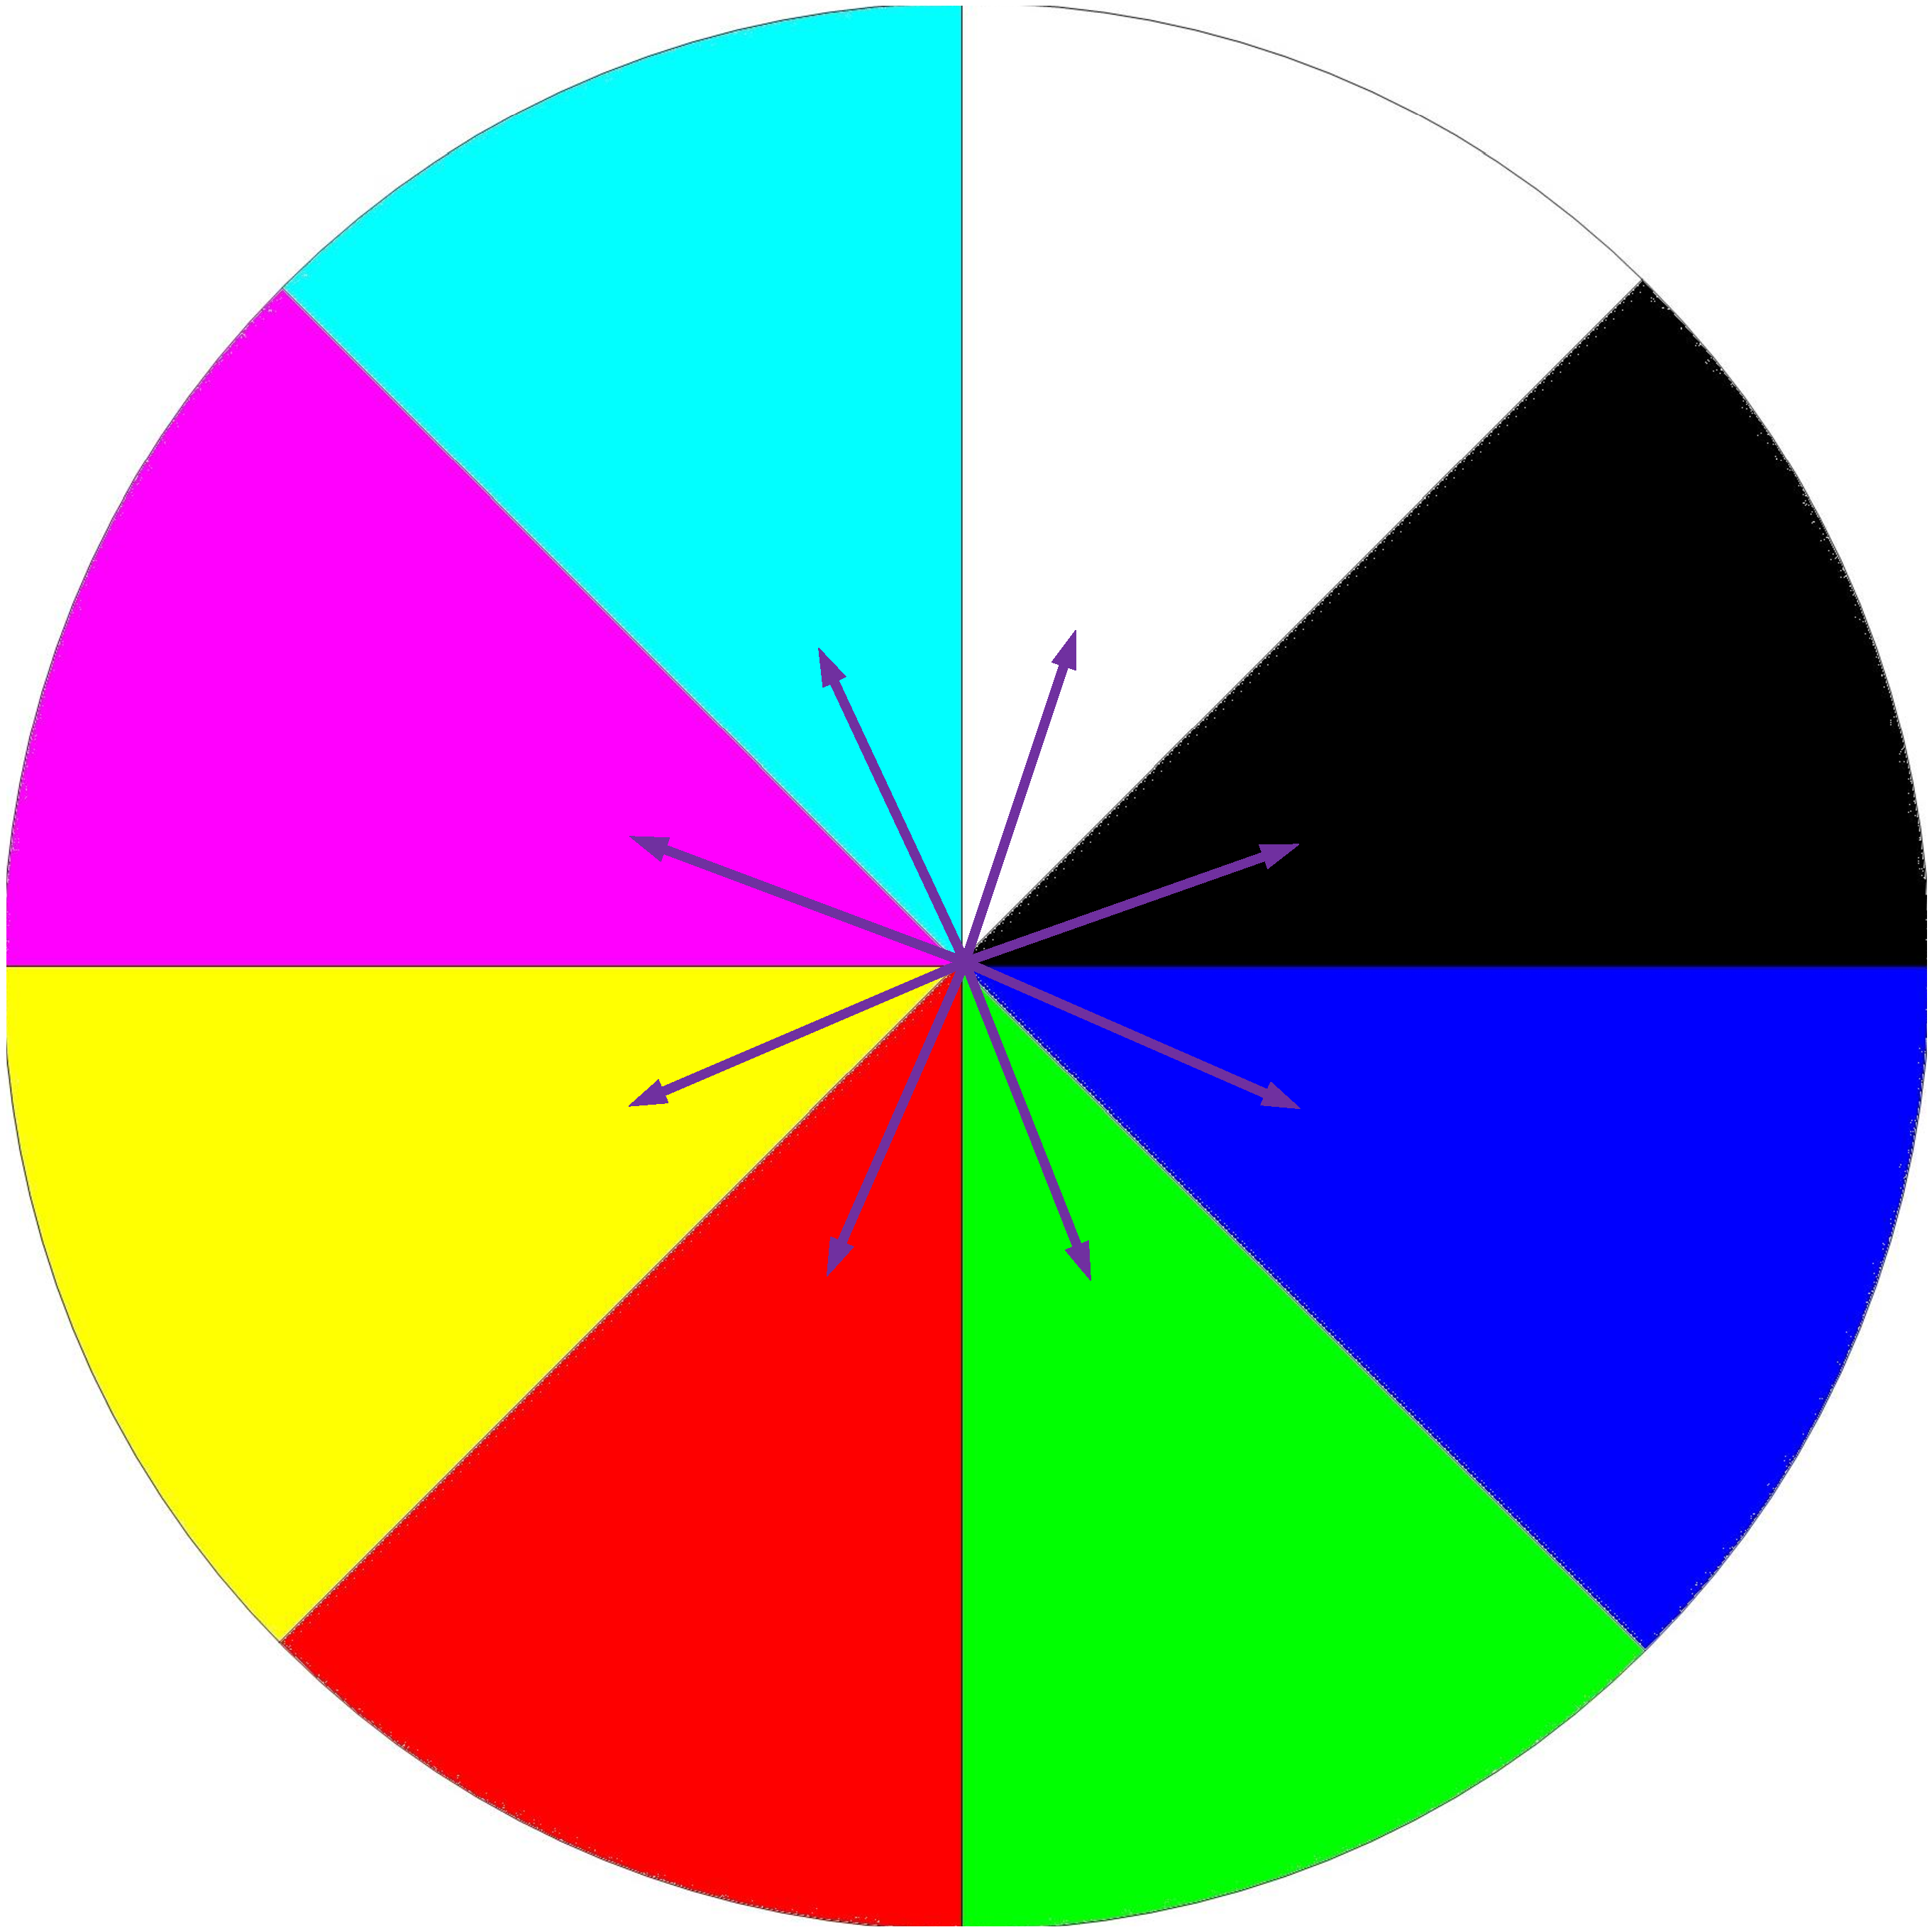
\includegraphics[width=3cm, height=3cm]{figures/8directions2-crop.pdf}}
	\caption[Typical activities in QMUL Junction Dataset]
	{(1)- (22) are typical activity patterns discovered by HDP models. The activities are sorted according to the number of the words assigned by the training corpus (in a descending order). (23) is the manually labeled legal vehicles driving lanes (red lines) and pedestrians walking lanes (yellow dash lines). The motion is quantified into eight directions and labeled in eight colors as (24).}
	\label{qmul_activity}
\end{figure}



\section{Dataset}
\label{dataset}
Three benchmark datasets were adopted in our experiment to evaluate our proposed method. Each of them is captured from a complicated crowded traffic junction, which is regulated by the traffic lights. Their details are listed as follows
\begin{itemize}
	\item[1]\textbf{QMUL Junction Dataset} \cite{hospedales2009markov}: This contains 1 hour of 25 fps video (90000 frames) with frame size $360\times288$. The video covers a busy traffic junction containing three major flows in different directions. 
	\item[2]\textbf{QMUL Junction Dataset 2} \cite{hospedales2009markov}: This video length is 52 minutes with 25 fps (78000 frames). The frame size is $360\times288$. This video is captured in a busy street with particularly busy pedestrian activity. 
	\item[3]\textbf{MIT Dataset}~\cite{wang2009unsupervised}: It consists of 1.5 hour of 30fps (162000 frames) with frame size $720\times 480$, and captures a far-field traffic scene.
\end{itemize}

\section{Parameter Setting}
\label{parameter}
To construct the codebook of visual words, we spatially divided the image scene into square cells of size $8\times8$. 
The local motions were quantified into eight directions as shown in~Fig.~\ref{fig:directions}. Therefore, the codebooks of both QMUL datasets have $12960$ words, while MIT contains $43200$ words. Each dataset was temporally segmented into non-overlapping video clips with $75$ frames. The threshold for optic flow estimation was 0.8.

For each dataset, the first 500 video clips (about 25 minute's length) were employed to learn the typical activities and traffic states. The rest of the video sequences were employed to simulate online screened video to test online performance, i.e., 699 clips of QMUL Junction Dataset, 539 clips of QMUL Junction Dataset 2 and 1711 clips of MIT Dataset were used for test.

The ARD kernel was adopted in both GP regression models and GP classification models. Their hyper-parameters were optimized by \emph{Conjugate Gradient} \cite{nocedal2006numerical}. The \emph{Laplace's } approximation method \cite{williams1998bayesian} was applied in GP classification models.

To infer the latent variables in HDP and HDP-HMM models, we exploited Gibbs sampling schemes for 1000 iterations. For the selection of their hyper-parameters $(\beta,\alpha)$, we performed a grid search on $\beta, \alpha\in \{0.1, 0.5, 1.0, 2.0\}$. 
We found that, even though the number of clusters increased with larger $\beta$ and $\alpha$, the numbers of typical activities and states always converged when at least $90\%$ of the total motions were explained. These numbers kept consistent when $\beta$ and $\alpha$ were both larger than 0.5. The additional clusters were generated to explain very rare motions. In this thesis, we were only interested in typical activities and states and we did not use topic models to estimate likelihood or posterior. Therefore, we did not need precise hyper-parameters. The hyper-parameters were fixed at $\beta = 2, \alpha=0.5$ for all experiments. In actual implementation of HDP and HDP-HMM models, the hyper-parameters can be optimized by giving a vague gamma prior and sampling them using the scheme proposed in~\cite{teh2006hdp}.


\section{Experiment on QMUL Junction Dataset}
\label{exp:qmul}
In this section, we will specially analyze the experimental process and results on QMUL Junction Dataset. The experimental results will be compared with others provided by some popular methods. Then, the experimental results on the other two datasets will be briefly illustrated and discussed.

\subsection{Learning Typical Activities and States}
\label{exp:qmul:activity_and_state}


The HDP models automatically learned 32 activities in this traffic scene, among which 22 were selected as typical activities, as shown in Fig.~\ref{qmul_activity}. Their corresponding percentages of how many words in the training corpus are assigned to them are noted. For a better illustration, we manually painted all possible motion flows for vehicles and pedestrians and marked them with alphabetic letters in~Fig.~\ref{fig:subfigure:qmul_path}. Each path is explained as follows:

\begin{figure}[!htbp]
	\renewcommand{\thesubfigure}{\arabic{subfigure}}
	%\renewcommand{\thefigure}{\arabic{figure}}
	\makeatletter
	\renewcommand{\@thesubfigure}{(\thesubfigure)\space}
	\renewcommand{\p@subfigure}{\thefigure.}
	\makeatother
	\centering
	\centering
	\subfigure[0.38\%]{
		\label{fig:subfigure:23}
		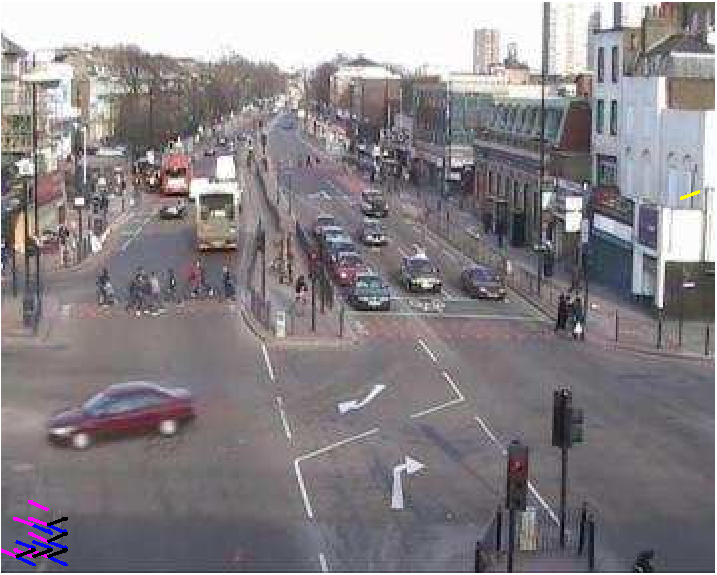
\includegraphics[width=3.7cm, height=2.5cm]{figures/qmul/t23-crop.pdf}}
	\subfigure[0.08\%]{
		\label{fig:subfigure:24}
		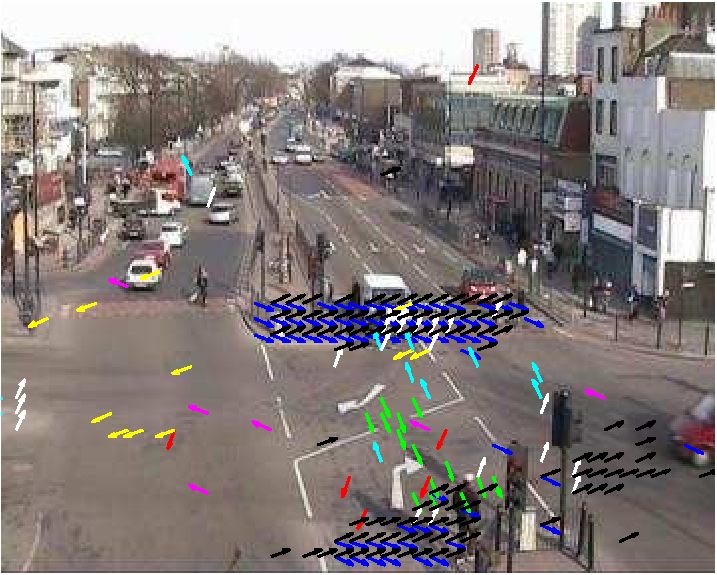
\includegraphics[width=3.7cm, height=2.5cm]{figures/qmul/t24-crop.pdf}}
	\subfigure[0.08\%]{
		\label{fig:subfigure:25}
		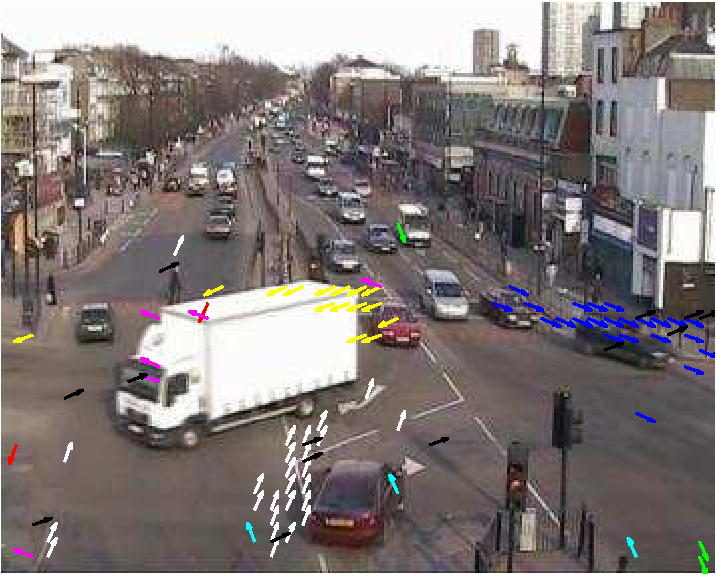
\includegraphics[width=3.7cm, height=2.5cm]{figures/qmul/t25-crop.pdf}}
	\subfigure[0.03\%]{
		\label{fig:subfigure:26}
		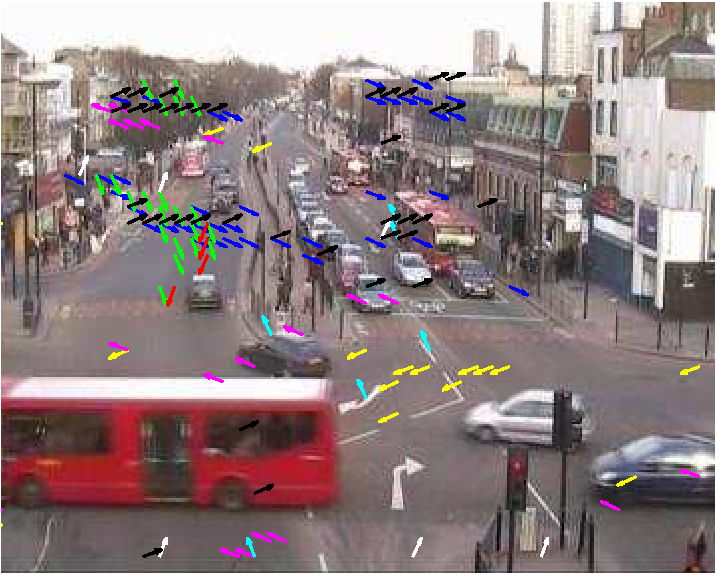
\includegraphics[width=3.7cm, height=2.5cm]{figures/qmul/t26-crop.pdf}}
	\subfigure[0.03\%]{
		\label{fig:subfigure:27}
		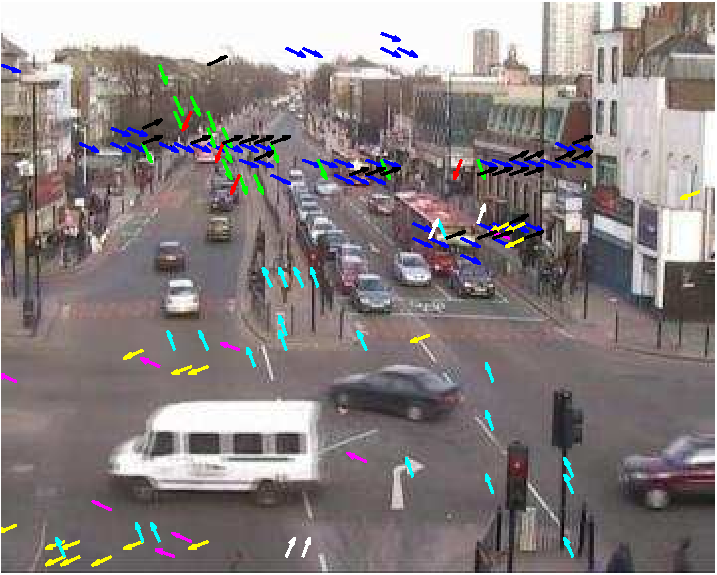
\includegraphics[width=3.7cm, height=2.5cm]{figures/qmul/t27-crop.pdf}}
	\subfigure[0.02\%]{
		\label{fig:subfigure:28}
		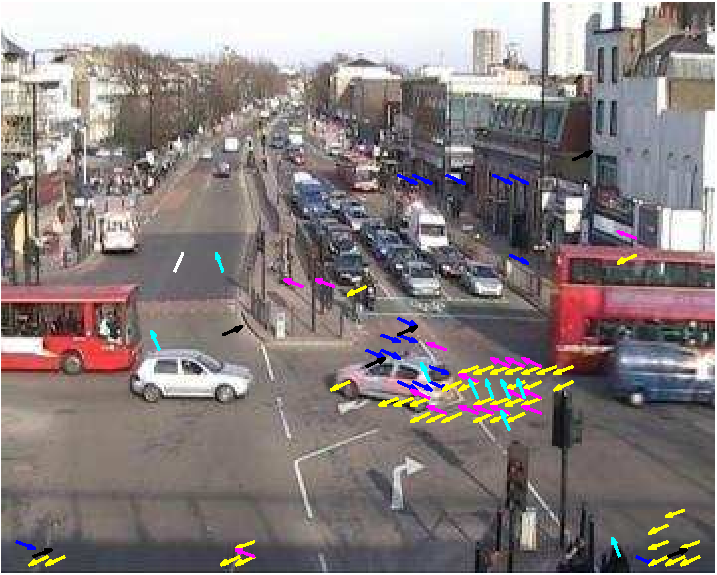
\includegraphics[width=3.7cm, height=2.5cm]{figures/qmul/t28-crop.pdf}}
	\subfigure[0.01\%]{
		\label{fig:subfigure:29}
		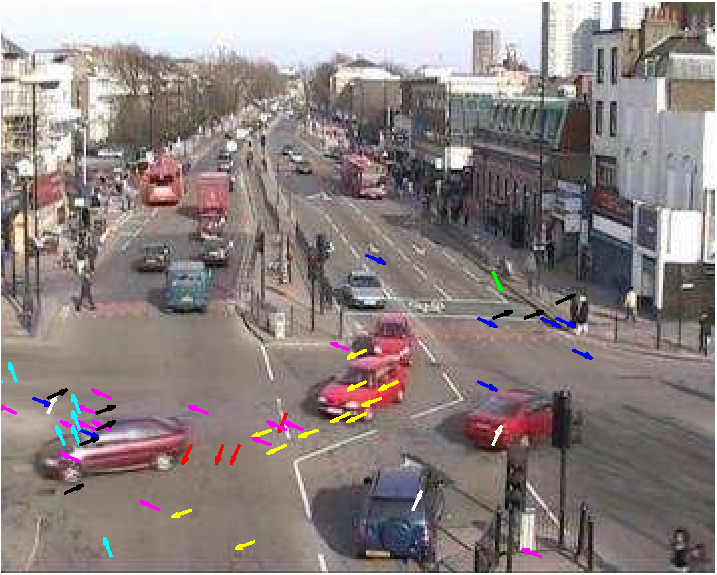
\includegraphics[width=3.7cm, height=2.5cm]{figures/qmul/t29-crop.pdf}}
	\subfigure[0.01\%]{
		\label{fig:subfigure:30}
		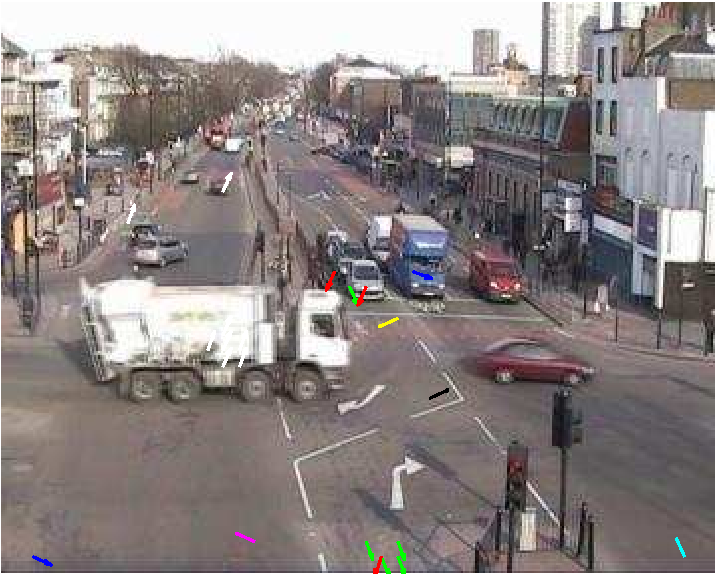
\includegraphics[width=3.7cm, height=2.5cm]{figures/qmul/t30-crop.pdf}}
	\caption[Rare activities in QMUL Junction Dataset]
	{8 rarely occurring activities.}
	\label{fig:rare_activity}
\end{figure} 


\begin{figure}[!htp]
	\subfigure[Vertical flow]{
		\begin{minipage}{0.45\linewidth}
			\centering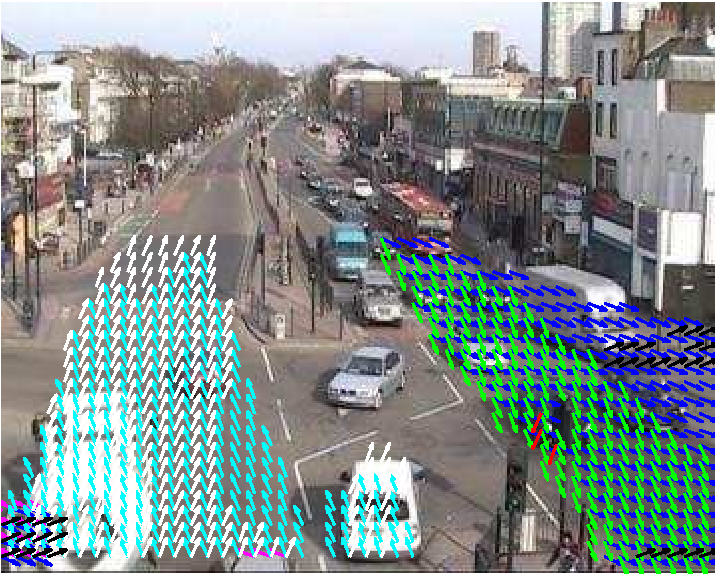
\includegraphics[width = 4cm]{figures/qmul/ss1-crop.pdf}\\
			\vfill
			\centering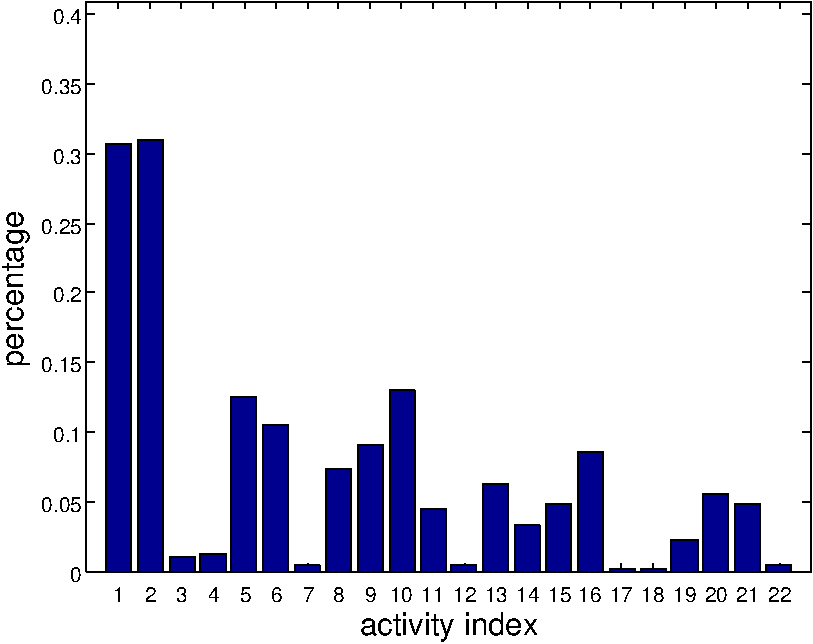
\includegraphics[width = 5.2cm]{figures/qmul/hist_s1-crop.pdf}
		\end{minipage}
		\label{fig:subfigure:state1}
	}
	\hfill
	\subfigure[Leftward flow]{
		\begin{minipage}{0.45\linewidth}
			\centering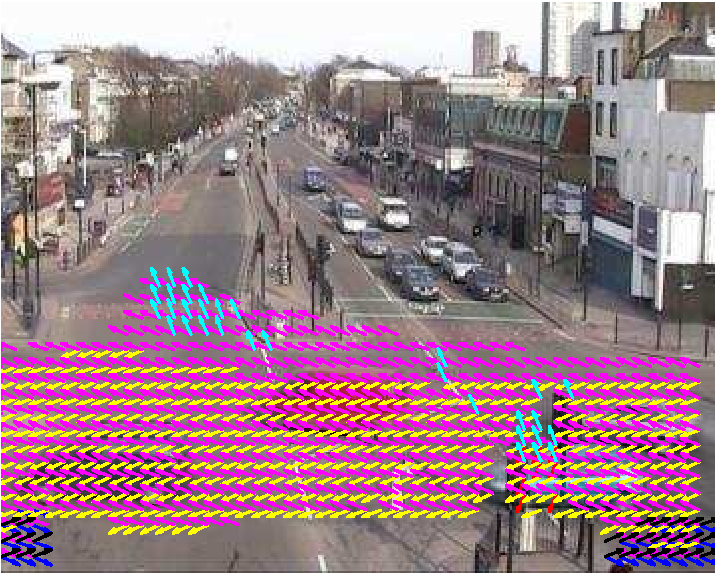
\includegraphics[width = 4cm]{figures/qmul/ss3-crop.pdf}\\
			\vfill
			\centering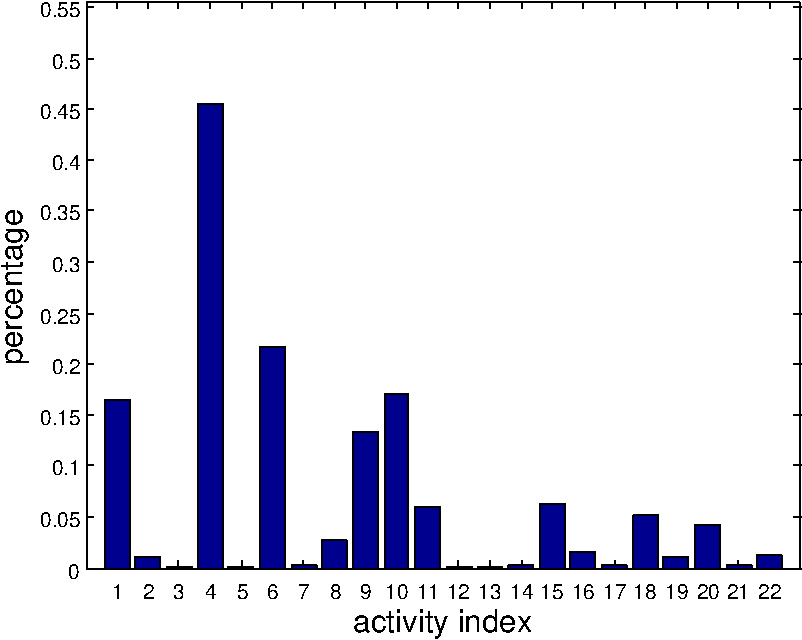
\includegraphics[width = 5.2cm]{figures/qmul/hist_s3-crop.pdf}
		\end{minipage}
		\label{fig:subfigure:state2}
	}
	\hfill
	\subfigure[Rightward flow]{
		\begin{minipage}{0.45\linewidth}
			\centering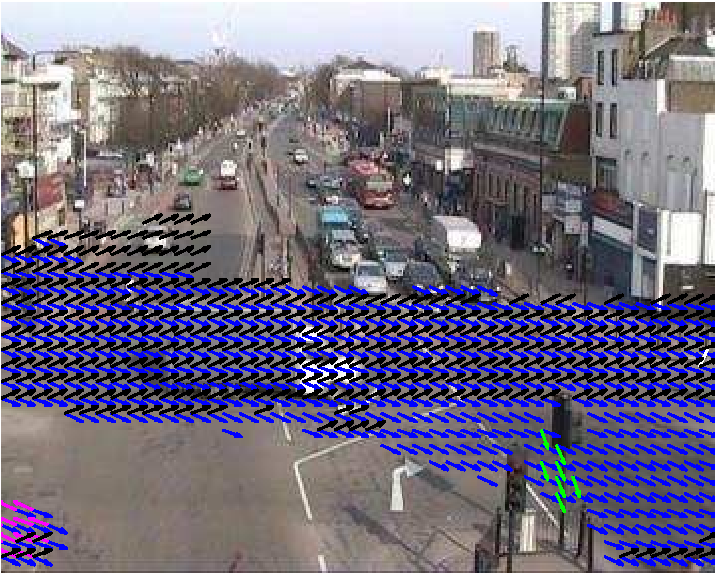
\includegraphics[width = 4cm]{figures/qmul/ss2-crop.pdf}\\
			\vfill
			\centering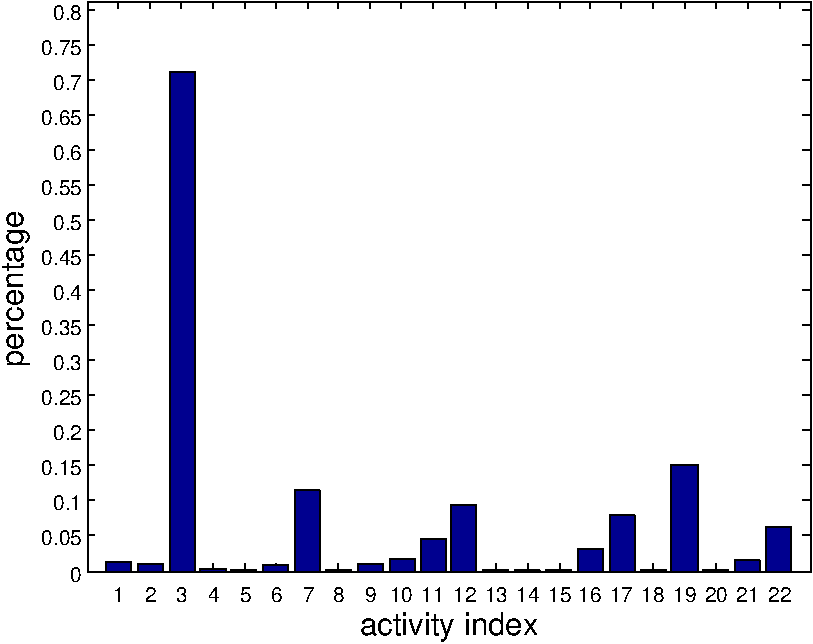
\includegraphics[width = 5.2cm]{figures/qmul/hist_s2-crop.pdf}
		\end{minipage}
		\label{fig:subfigure:state3}
	}
	\hfill
	\subfigure[Left and right turn]{
		\begin{minipage}{0.45\linewidth}
			\centering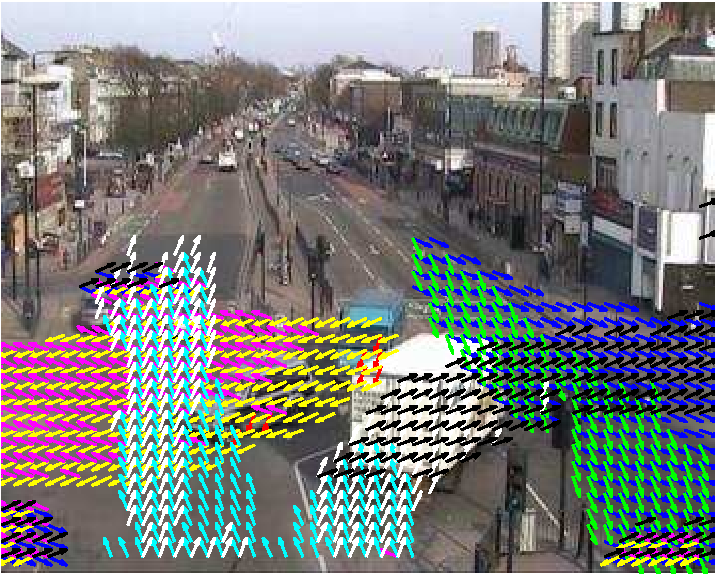
\includegraphics[width = 4cm]{figures/qmul/ss4-crop.pdf}\\
			\vfill
			\centering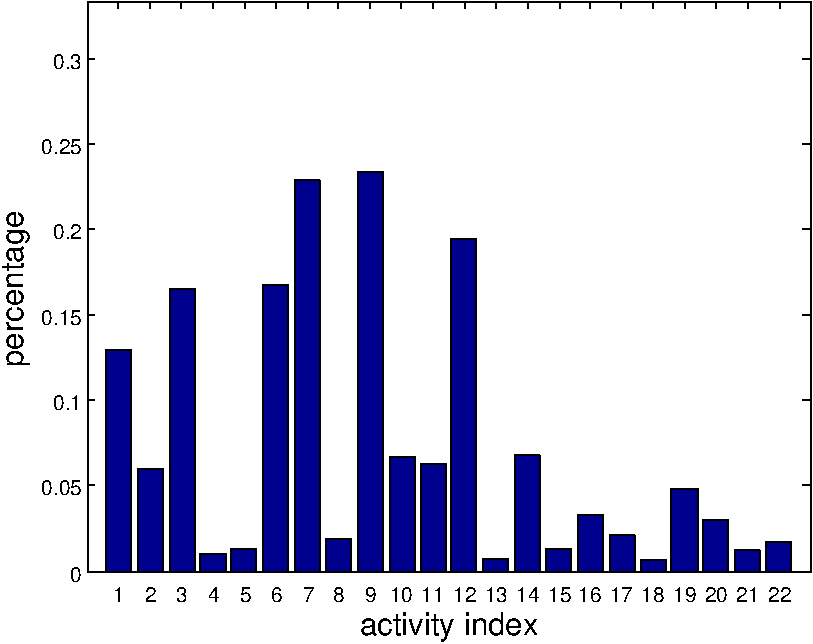
\includegraphics[width = 5.2cm]{figures/qmul/hist_s4-crop.pdf}
		\end{minipage}
		\label{fig:subfigure:state4}
	}		
	\caption[Typical traffic states in QMUL Junction Dataset]{4 typical traffic states are learned by HDP-HMM model. The states are sorted according to the traffic light cycle. Their corresponding average mixtures of typical activities throughout the training set are shown in the histograms. The x-axis is the index of atomic activities and the y-axis is the percentage of each atomic activity.}
	\label{qmul_state}
\end{figure}

\begin{itemize}
	\item Flow a: Vehicles driving upward from bottom in the left traffic lane. Topic 2, 5, 13 and 21 form this flow.
	\item Flow b: Vehicles driving downward from top in the left traffic lane. It is mainly explained by topics 1, 8 and 20. Part of topic 10 also covers this flow.
	\item Flow c: Vehicles from top turning left. It can be explained by topics 6 and 20.
	\item Flow d: Vehicles turning left from the left entrance. It is explained by the upper part of topic 4.
	\item Flow e: Vehicles in the left bottom corner turning left, as shown in topic 16.
	\item Flow f: Vehicles from top making a right turn in the middle of the junction, as shown in topics 12 and 7.
	\item Flow g: Vehicles from bottom making a right turn in the middle of the junction. Topic 14 is its first step: vehicles driving into the middle area from bottom and waiting for time to make a right turn as topic 9.
	\item Flow h (leftward) and i: Vehicles driving leftward and part of them making a right turn. It is dominated by topic 3, 7 and 19. Topic 17 also explains such flow caused by high vehicles such as double-decker buses.
	\item Flow h (rightward) and j: Vehicles driving rightward and part of them making a right turn. It mainly consists of topics 4, 6 and 10. Topics 15 and 18 also explain such flow caused by high vehicles.
	\item Flow k and l: Pedestrian crossing the road in topics 15 and 18 rightward and in topic 17 leftward.
	\item Flow m: People crossing the road in the right bottom corner. %\subsection{Abnormality Detection}
\end{itemize}



Fig.~\ref{fig:rare_activity} shows the 8 rarely occurring activities learned by the HDP models. From the figure we can see, some of them are caused by rarely occurring abnormal events: in Fig.~\ref{fig:subfigure:24} the people is walking in the area for vehicles (middle bottom); Fig.~\ref{fig:subfigure:28} is caused by a police car diving reversely ; Fig.~\ref{fig:subfigure:26} shows something crossing the left lane where for vehicles driving upward. Motions distribute in the other rare activity patterns in chaos. They are caused by noise or lighting changing.

The HDP-HMM models automatically learned 9 traffic states. We selected 4 of them as typical states, which have the highest percentage among all clips, as shown in Fig.~\ref{qmul2_state}. Their corresponding average feature vectors over the training set are shown below them. Each state is explained as follows:
\begin{itemize}
	\item Vertical flow: Topics 1 and 2 dominate in this interaction. The other topics such as 5, 8 and 10 related to vertical traffic topics have also relative high values in the histogram.
	\item Leftward flow: It mainly consists by topics 4, 6 and 10. Topics 1, 8 and 9 overlap this flow. The feature values of topics 15 and 18 are relative high because of pedestrians.
	\item Rightward flow: It is absolutely dominated by topic 3. Topics 7, 12, 17 and 19 are also important components. The feature values of topics 11, 17 and 22 are relative high because of pedestrians.
	\item Left and right turn: This state happens during the state of vertical flow, when the vertical flow temporally terminates. It is a complicated interaction among a couple of topics, such as topics 1, 3, 6, 7, 8 and 12.
\end{itemize}

\begin{figure}[!htbp]
	\centering
	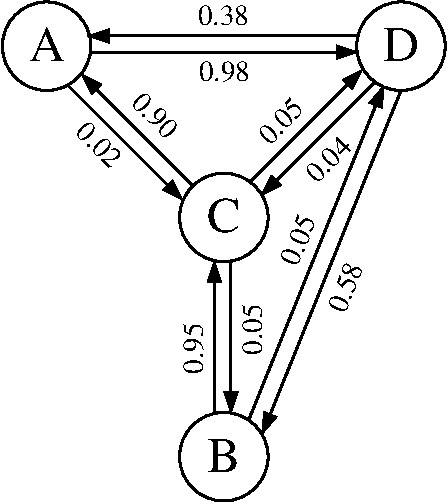
\includegraphics[width=5cm]{figures/transition_qmul-crop.pdf}
	\caption[State transition graph of QMUL Junction Dataset]{State transition graph for QMUL Junction Dataset. The arrow indicates the transition direction and the number denote the transition probability.}
	\label{fig:qmul_transition}
\end{figure}

Fig.\ref{fig:qmul_transition} illustrates the state transition directions (arrows) and the corresponding transition probabilities. From the graph we can see, the transition is in a strict order. However, there is still a very low probability for the transition from state A to C (0.02), C to B (0.05) and B to D (0.05). It might be caused by emergency vehicles cutting off current state and changing it, or some training video clips being falsely clustered by HDP-HMM models.


\subsection{Online Classifying Traffic States}
\label{exp:qmul:online classify} 
We used the rest part of the video sequence (699 clips) to simulate the online classification task.
Each 75 newly screened video frames were segmented into a clip.
%The online screened video stream was segmented into clips of 75 frames each. 
Then the high-level features were extracted to represent the state in this clip. 
Using our classifier it was assigned with one of the four state labels.
Fig.~\ref{fig:online_exsample_qmul} shows an example for each traffic state that was recognized in 4 clips from online capture video sequence, respectively. Their corresponding high-level features $\mathbf{c}_t =\{p_{t1},\cdots,p_{tK}\}$ are illustrated below. For comparison, the mean features' value of each state are marked by the red curves.
To lively illustrate the construction of an interaction during a clip, the interaction in Fig.~\ref{fig:s4_exsample} is decomposed into 5 main typical activities, as shown in Fig.~\ref{fig:qmul:interaction_decomposition}. 

We have manually labeled each clip to validate the classification results by our model. The confusion matrix is shown in Tab.~\ref{tab:qmul_confuse}. From the matrix we see that, our model have a very high classification accuracy. 4 clips are falsely classified as shown in Fig.~\ref{fig:qmul_falsely_classified}. Even with the help of transition information these wrong results can be modified. Fig.~\ref{fig:qmul_classification_result} shows the labels of the 699 test video clips. Note the periodicity of the labels assigned. We can observe that each traffic cycle lasts around 40 clips i.e. 120 seconds.
We have also compared our classification results with those generated by popular methods in Tab.~\ref{tab:qmul_compare}. From the table we see that our model outperforms other three popular methods in terms of classification results. 
Notice that, this comparison is for your information only. 
Normally, the learned traffic states are different by using different methods. Our method has learned the same traffic states in this dataset as others by chances, because the main traffic state in this scene are very explicit. On the other side, different studies often adopt different length of video clips, such as ours is 75 frames each clip while in~\cite{hospedales2009markov} was 25 frames and in~\cite{wang2009unsupervised} was 300 frames. It might leads to different results. We have not implemented others methods to achieve results under the same conditions of our experiments.
Therefore, for objective comparison and evaluation, we will not compare our method with the others in the other two datasets any more.
\begin{table}[!htbp]
	\begin{center}
		\renewcommand\arraystretch{2}
		\setlength{\tabcolsep}{8pt}
		\begin{tabular}{c c|c|c|c|c|}
			\multicolumn{1}{c}{ }	& \multicolumn{5}{c}{Our Classification }\\
			\multirow{5}{5pt}{\rotatebox{90}{Manually label}}		&\multicolumn{1}{c}{ }	&\multicolumn{1}{c}{a}	&\multicolumn{1}{c}{b}	&\multicolumn{1}{c}{c}	&\multicolumn{1}{c}{d}\\
			\cline{3-6}
			&a		&367	&0	&0	&0\\
			\cline{3-6}
			&b		&0	&143	&0	&1\\
			\cline{3-6}
			&c		&0	&0	&120	&0\\
			\cline{3-6}
			&d		&3	&0		&0	&64\\
			\cline{3-6}
		\end{tabular}
	\end{center}
	\caption[The confusion matrix of QMUL Juction Dataset]
	{The confusion matrix of QMUL Juction Dataset}
	\label{tab:qmul_confuse} 
\end{table}


We want to point it out that more clips would be falsely classified if only using the GP classifier. Fig.~\ref{fig:qmul_revised_detect} shows an example that the clip 667 was classified into state D but its previous clip was in state B and its following clip was state C. Hence, clip 667 should be the end of state B. According to the state transition graph (see Fig.~\ref{fig:qmul_transition}), transition probability from state B to state C is only 0.05. Hence, the classification result was corrected as state B by our model.

\begin{landscape}
	\begin{table}[!htbp]
		\begin{center}
			\renewcommand\arraystretch{1.5}
			\setlength{\tabcolsep}{7pt}
			\begin{tabular}{l | c c c c | c c c c | c c c c | c c c c}
				\toprule[1pt] 
				\multirow{2}{*}{State}		&\multicolumn{4}{c|}{MCTM}	&\multicolumn{4}{c|}{LDA}	&\multicolumn{4}{c|}{HMM}		&\multicolumn{4}{c}{Ours}\\
				\cmidrule{2-5}		\cmidrule{6-9}		\cmidrule{10-13}	\cmidrule{14-17}
				&L	&R	&V	&VT	&L	&R	&V	&VT	&L	&R	&V	&VT	&L	&R	&V	&VT\\
				\midrule[1pt]
				Left	&\textbf{.99}	&.00	&.00	&.01	&\textbf{.49}	&.44	&.00	&.06	&\textbf{.98}	&.00	&.01	&.01	
				
				&\textbf{1.0}	&.00	&.00	&.00\\
				
				Right	&.00	&\textbf{.94}	&.01	&.05	&.00	&\textbf{1.0}	&.00	&.00	&.00	&\textbf{.92}	&.08	&.00	
				
				&.00	&\textbf{.99}	&.00	&.01\\
				
				Vertical	&.00	&.00	&\textbf{.77}	&.22	&.01	&.17	&\textbf{.82}	&.00	&.02	&.01	&\textbf{.69}	&.28	
				
				&.00	&.00	&\textbf{1.0}	&.00\\
				
				Vertical-Turn	&.31	&.05	&.20	&\textbf{.43}	&.01	&.21	&.30	&\textbf{.46}	&.49	&.04	&.32	&\textbf{.15}	
				
				&.05	&.00	&.00	&\textbf{.95}\\
				\cmidrule{1-17}	
				Average Accuracy		&\textbf{.78}	&	&	&	&\textbf{.69}	&	&	&	&\textbf{.69}	&	&	&	
				
				&\textbf{.99}	&	&	&\\	%[5ex]
				
				\bottomrule[1pt] 
				
			\end{tabular}
		\end{center}
		\caption[Comparison of Classification results between our methods and others popular methods for QMUL Juction Dataset]
		{Comparison of Classification results between our methods and others popular methods for QMUL Juction Dataset: The results of MCTM, LDA and HMM are cited from ~\cite{hospedales2012video}}
		\label{tab:qmul_compare} 
	\end{table}
\end{landscape}



\clearpage
\newpage
\begin{figure}[!htbp]
	\subfigure[Vertical flow]{
		\begin{minipage}{0.45\linewidth}
			\centering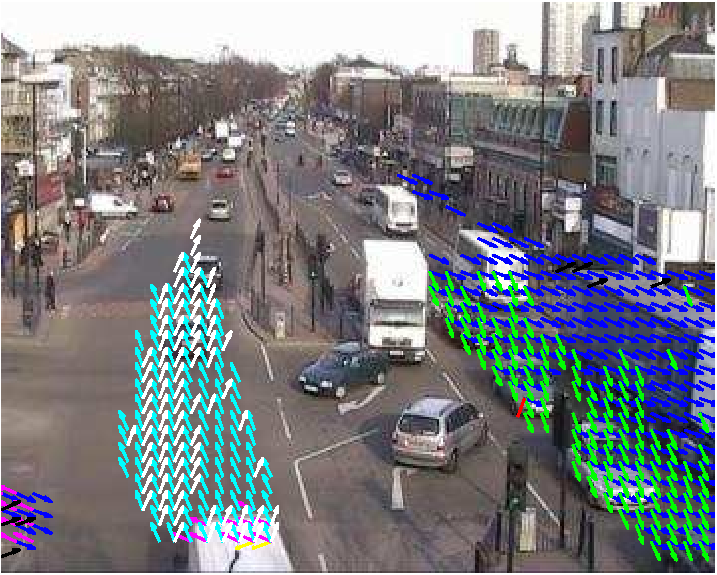
\includegraphics[width = 5cm]{figures/qmul/s3_example_686-crop.pdf}\\
			\vspace{0.3cm}
			\centering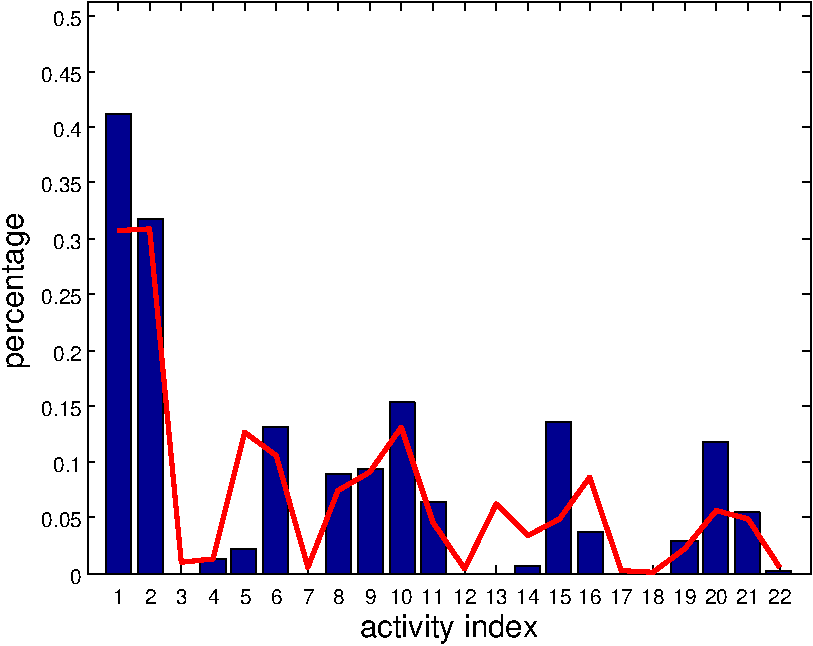
\includegraphics[width = 6.5cm]{figures/qmul/s3_example_hist_686-crop.pdf}
		\end{minipage}
		\label{fig:s3_exsample}
	}
	\hfill
	\subfigure[Leftward flow]{
		\begin{minipage}{0.45\linewidth}
			\centering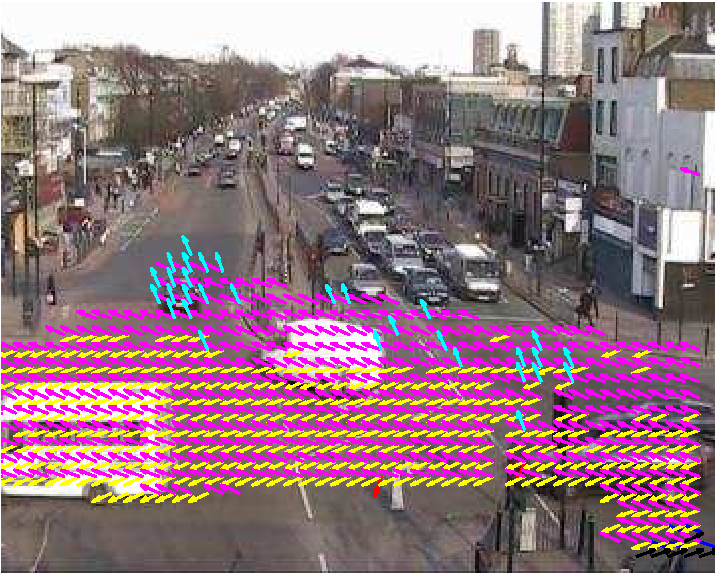
\includegraphics[width = 5cm]{figures/qmul/s4_example_699-crop.pdf}\\
			\vspace{0.3cm}
			\centering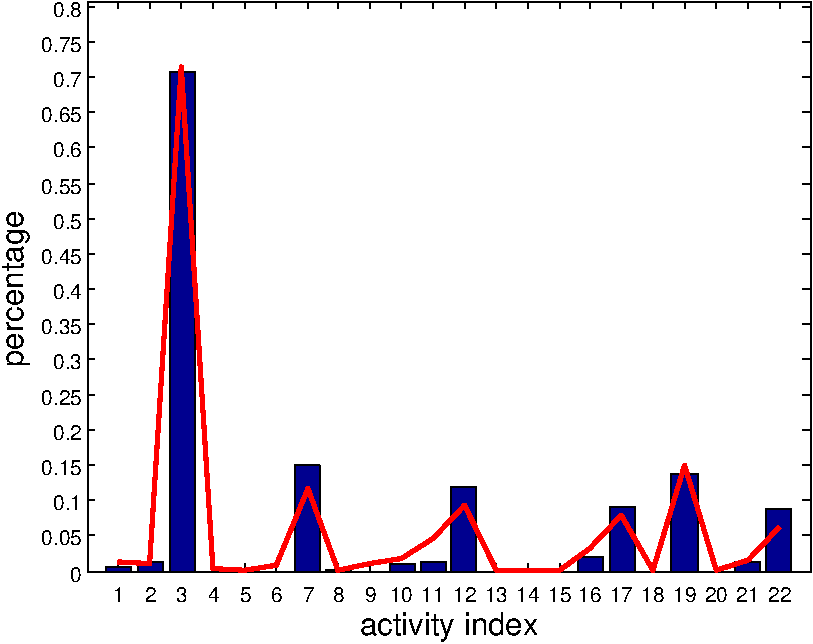
\includegraphics[width = 6.5cm]{figures/qmul/s4_example_hist_699-crop.pdf}
		\end{minipage}
		\label{fig:s4_exsample}
	}
	\hfill
	\subfigure[Rightward flow]{
		\begin{minipage}{0.45\linewidth}
			\centering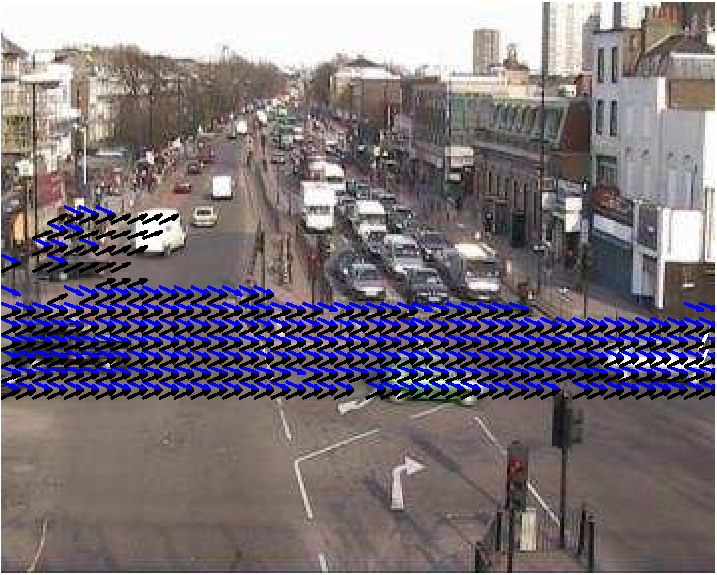
\includegraphics[width = 5cm]{figures/qmul/s1_example_708-crop.pdf}\\
			\vspace{0.3cm}
			\centering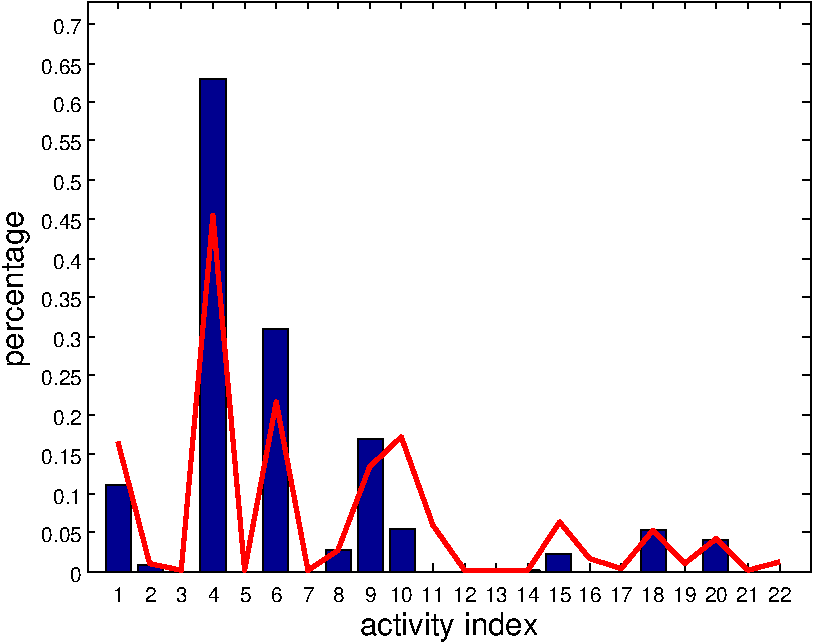
\includegraphics[width = 6.5cm]{figures/qmul/s1_example_hist_708-crop.pdf}
		\end{minipage}
		\label{fig:s1_exsample}
	}
	\hfill
	\subfigure[Left and right turn]{
		\begin{minipage}{0.45\linewidth}
			\centering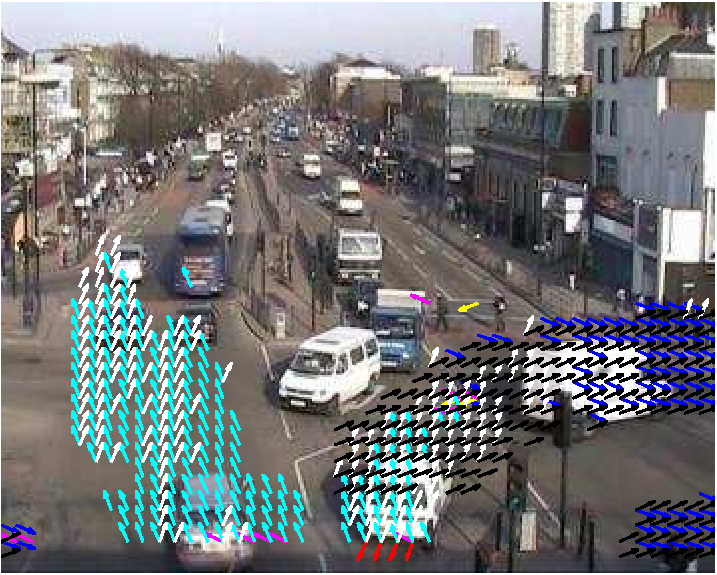
\includegraphics[width = 5cm]{figures/qmul/s8_example_832-crop.pdf}\\
			\vspace{0.3cm}
			\centering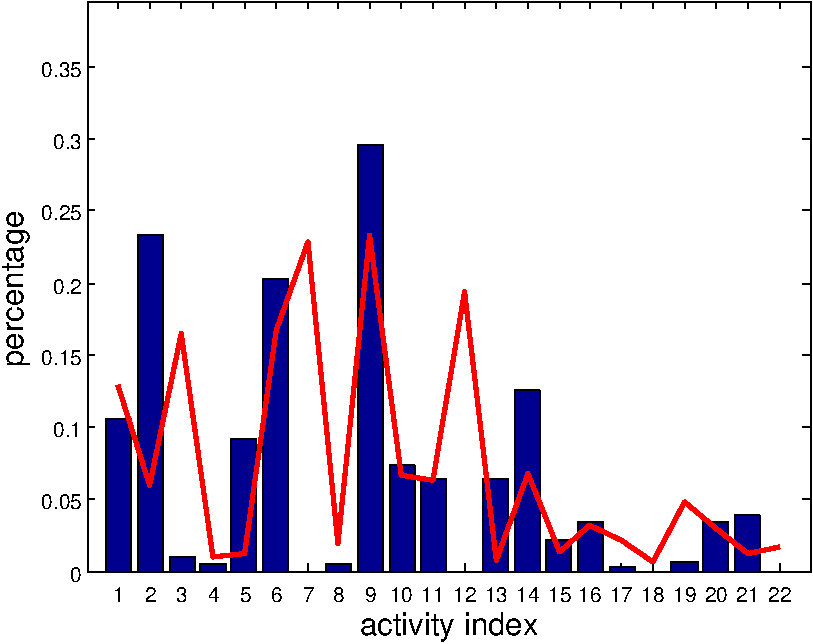
\includegraphics[width = 6.5cm]{figures/qmul/s8_example_hist_832-crop.pdf}
		\end{minipage}
		\label{fig:s8_exsample}
	}
	\caption[Examples of online classification in QMUL Junction Dataset]
	{We show a video clip as an example for each type of traffic state in the first row. Their corresponding features histograms are shown in the second row. For comparison, the red curve in each plot is the average activity mixture over the training video.}
	\label{fig:online_exsample_qmul}
\end{figure}

\clearpage
\newpage
\begin{landscape}
	\begin{figure}[!htbp]
		\centering
		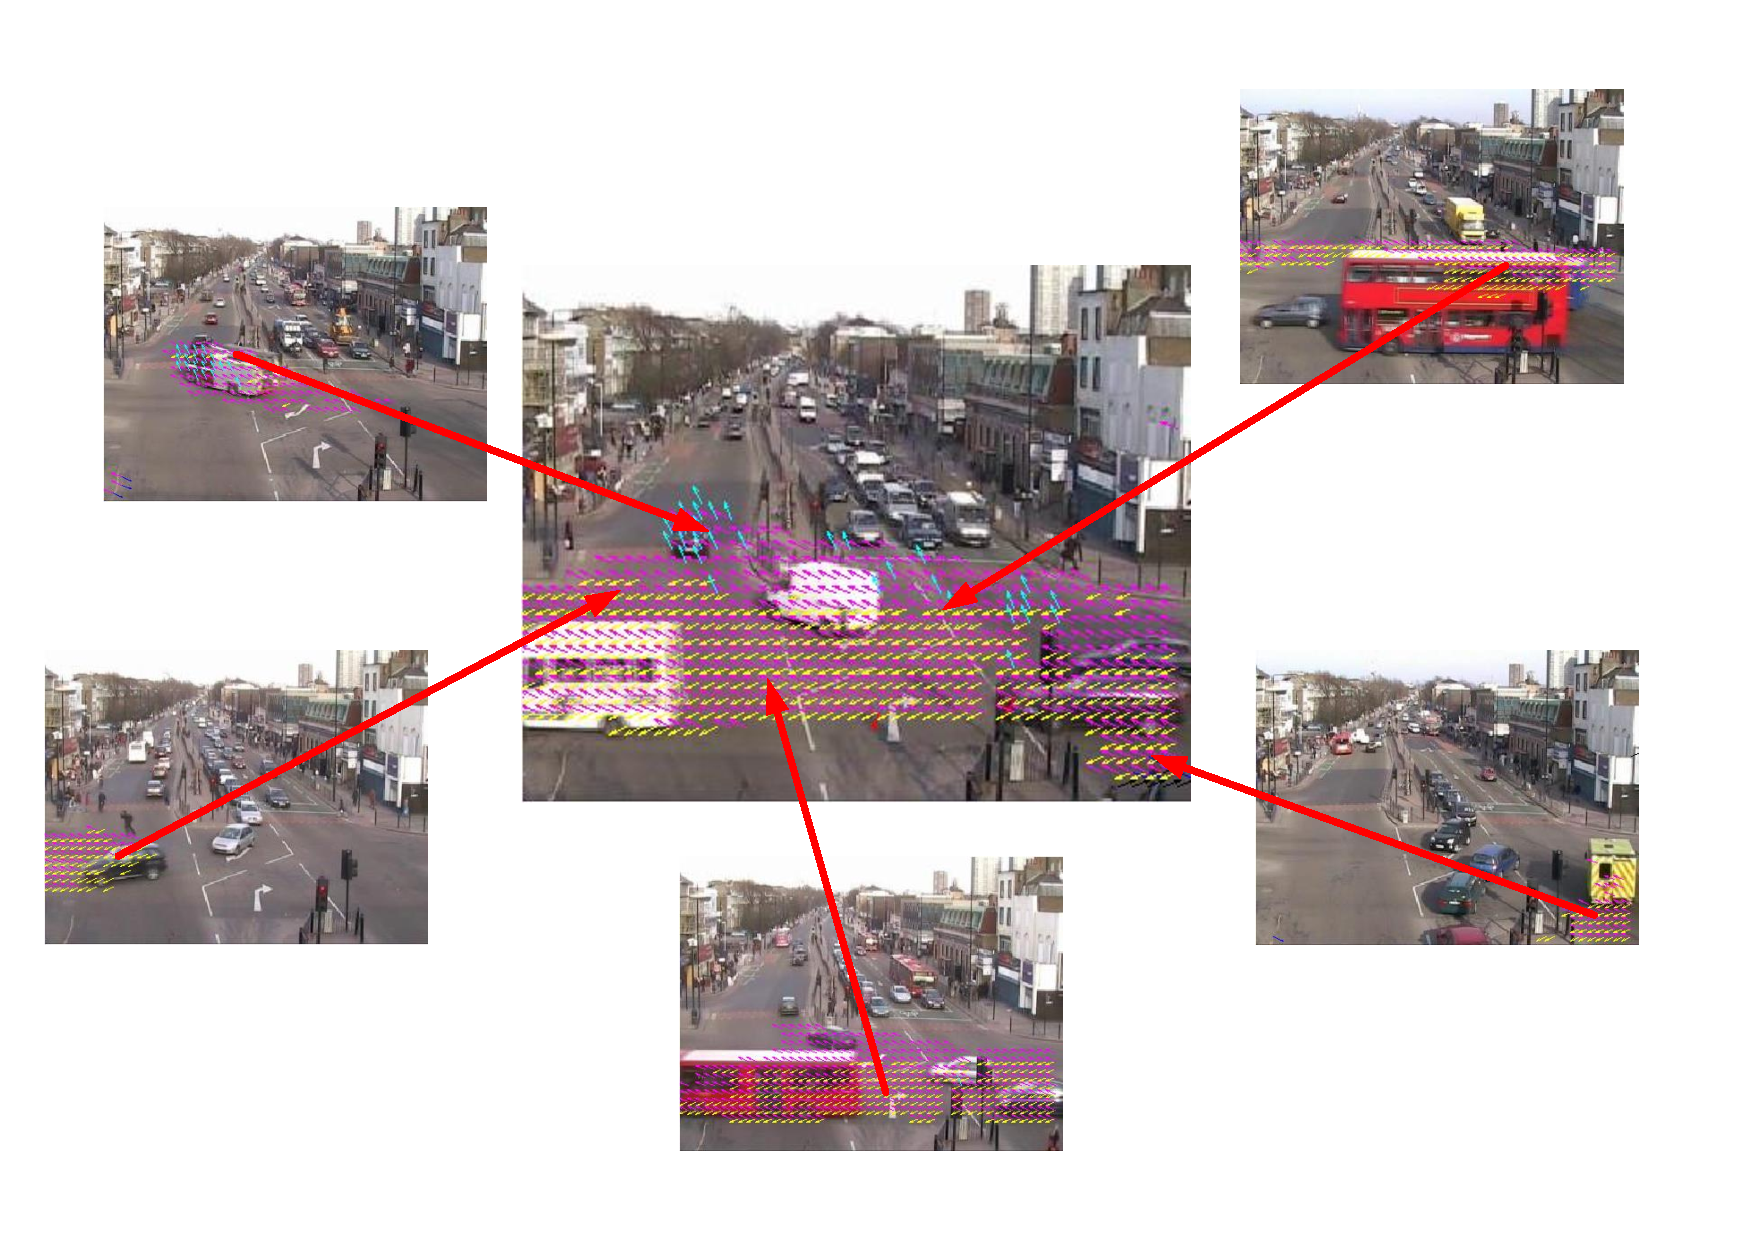
\includegraphics[width = 20cm]{figures/qmul/construct_example_699_new.pdf}
		\caption[Decomposition of an interaction into main activities]
		{The interaction in the video clip Fig.~\ref{fig:s4_exsample} is decomposed into five main activities.}
		\label{fig:qmul:interaction_decomposition}
	\end{figure}
\end{landscape}

\begin{figure}[!htbp]
	\centering
	\subfigure[]{
		\includegraphics[width = 5.5cm]{figures/qmul/falsedetect/542_s3s8-crop.pdf}
	}\hspace{1cm}
	\subfigure[]{
		\includegraphics[width = 5.5cm]{figures/qmul/falsedetect/543_s3s8-crop.pdf}
	}
	\subfigure[]{
		\includegraphics[width = 5.5cm]{figures/qmul/falsedetect/617_s3s8-crop.pdf}
	}\hspace{1cm}
	\subfigure[]{
		\includegraphics[width = 5.5cm]{figures/qmul/falsedetect/1043_s8s4-crop.pdf}
	}
	\caption[Falsely classified clips in QMUL Junction Dataset]{The four falsely classified clips in QMUL Junction Dataset.}
	\label{fig:qmul_falsely_classified}
\end{figure}

\begin{figure}[!htbp]
	\centering
	\subfigure[clip 666]{
		\includegraphics[width = 4cm]{figures/qmul/falsedetect/666_s4-crop.pdf}
	}
	\subfigure[clip 667]{
		\includegraphics[width = 4cm]{figures/qmul/falsedetect/667_s8s4-crop.pdf}
	}
	\subfigure[clip 668]{
		\includegraphics[width = 4cm]{figures/qmul/falsedetect/668_s1-crop.pdf}
	}
	\caption[Transition information corrected the falsely classified result by GP model]{An example for falsely classified result by GP model being corrected by using transition information.}
	\label{fig:qmul_revised_detect}
\end{figure}

\clearpage
\newpage
\begin{landscape}
	\begin{figure}[h]
		\centering
		\subfigure[ The classification results of 699 video clips]{
			\includegraphics[width = 22cm]{figures/qmul/qmul_state_sequence.png}
		}\\
		\subfigure[Zoom in of the classification result rom clip 400 to clip 520]{
			\includegraphics[width = 22cm]{figures/qmul/qmul_state_sequence_zoom.png}
		}
		\caption[Classification results of QMUL Junction Dataset]{Classification results of 699 video clips. In both histograms the x-axis is the index of video clips in temporal order and the y-axis is the label of the four traffic states shown in Fig.~\ref{qmul_state}}
		\label{fig:qmul_classification_result}
	\end{figure}
\end{landscape}


%%*****************************************************************************
%%=============================================================================
\clearpage
\newpage
\subsection{Abnormal Events Detection}
\label{exp:qmul:online classify} 
The three kinds of abnormal events were identified as discussed in Sec.~\ref{framework:abnormal}, respectively. In this QMUL Junction scene the main abnormal events include Jaywalking, illegal U-turn and emergencies caused by ambulances, fire engines and police cars. Some of the examples for each kind of abnormal event are illustrated as following. Fig.~\ref{fig:rare_motion_abnormalevents} illustrates the two abnormal events caused by rarely occurring motions. For example, the motions of the ambulance have never occurred in the training data Fig.~\ref{fig:qmul_ambulance}. The ambulance is driving in an absolutely forbidden direction in the lane.

\begin{figure}[!htbp]
	\centering
	\subfigure[Ambulance]{
		\includegraphics[width = 6cm, height=4.5cm]{figures/qmul/abnormal/ambulance_212.png}
		\label{fig:qmul_ambulance}
	}
	\hspace{1.5cm}
	\subfigure[Pedestrian walking in improper area]{
		\includegraphics[width = 6cm, height=4.5cm]{figures/qmul/abnormal/jw3_354.png}
		\label{fig:qmul_jaywalking1}
	}
	\caption[Abnormal Events caused by rarely occurring motions]{Abnormal Events caused by rarely occurring motions. In the training dataset such motions have rarely or never occurred. They do not belong to any typical activities. The red boxes highlight the abnormal agents.}
	\label{fig:rare_motion_abnormalevents}
\end{figure}

In Fig.~\ref{fig:illegal_transition}, the traffic state is forced to change in an illegal ordering due to the fire engine. 
The rightward flow should not follow the vertical flow according to the learning results by HDP-HMM models. Therefore, the  clip was identified as abnormal event, even though its appearance is definitely a right flow state.

\begin{figure}[!htbp]
	\centering
	\begin{minipage}{0.26\textwidth}
		\includegraphics[width=5cm]{figures/qmul/fireengine_412-crop.pdf}\\
		\centering\scriptsize{Vertical flow in $t-1$ clip}
	\end{minipage}
	\hspace{1cm}
	%\caption{Vertical flow in $t-1$ clip}
	\begin{minipage}{0.26\textwidth}
		\includegraphics[width=5cm]{figures/qmul/abnormal/fireengine_413.png}
		\centering\scriptsize{Fire engine presents in $t$ clip}
	\end{minipage}
	\hspace{1cm}
	%\caption{Fire engine present in $t$ clip}
	\begin{minipage}{0.26\textwidth}
		\includegraphics[width=5cm]{figures/qmul/abnormal/fireengine_414.png}
		\centering\scriptsize{Rightward flow in $t+1$ clip}
	\end{minipage}
	\caption[Abnormal Event caused by illegal state transition]{Abnormal Event caused by illegal state transition. A fire engine interrupts the current vertical flow. The red boxes highlight the abnormal agents. }
	\label{fig:illegal_transition}
\end{figure}

Normally, abnormal events are caused by conflicting activities like Jaywalking, illegal U-turn converse driving or aggressively cutting in other roads. 
We illustrate an example for each type of such conflicting activities in Fig~.\ref{fig:qmul:conflict_activities}. 
The conflicting activities were detected by our GP regression models as discussed in Sec.~\ref{framework:abnormal}. If the observed value (blue bar) of any activities is larger than its predicted value (green curve and circle) as $1.96\sigma$ (red curve and cross), it is judged as a conflict activity against the others. The abnormally acting agents are marked by red boxes. 
They are analyzed in detail as following (all the related atomic activities are founded in Fig.~\ref{qmul_activity}):
\begin{itemize}
	\item Fig.~\ref{fig:qmul_police1} and ~\ref{fig:qmul_police2} show the police car driving conversely.
	\item This counter flow induces the value of activities 3 and 17 in the former clip, activities 3 and 19 in the latter clip. 
	\item A fire engine cuts off the vertical flow (see Fig.~\ref{fig:qmul_fireengine1}) and causes the activity 4 much stronger than the prediction.
	\item In Fig.~\ref{fig:qmul_uturn} the activity 19 is abnormal because of a vehicle making an illegal U-turn. 
\end{itemize}

Fig.~\ref{fig:qmul_missdetec_abnorml} shows some missing detected abnormal events. Because our method is beyond detecting, the categories of activity agents are not considered. For example, if a pedestrian is walking along the path of vehicles, it will not be detected as an abnormality, as shown in Fig.~\ref{fig:qmul_missdetect_bike} and~\ref{fig:qmul_missdetect_people}. 
In Fig.~\ref{fig:qmul_missdetect_fireengine}, before the fire engine drives into the camera scene, all vehicles have stopped and wait for its pass. Therefore, there is no activity in conflict with the fire engine. The scene is classified as leftward state. Because of its previous state is the sate left and right turn, this transition is legal. That is why this emergency was undetected.
A car is making an illegal U-turn in Fig.~\ref{fig:qmul_missdetect_uturn}. However, its activity seems identical with others in the leftward state. Hence, it is also not identified as an abnormal activity. The detection and tracking based approaches would perform better in this case.

\begin{figure}[!htbp]
	\centering\
	\subfigure[]{
		\includegraphics[width = 4.7cm]{figures/qmul/abnormal/false_detect_805-crop.pdf}
		\label{fig:qmul_flase_detect1}
	}
	\subfigure[]{
		\includegraphics[width = 4.7cm]{figures/qmul/abnormal/false_detect_881-crop.pdf}
		\label{fig:qmul_flase_detect1}
	}
	\subfigure[]{
		\includegraphics[width = 4.7cm]{figures/qmul/abnormal/false_detect_920-crop.pdf}
		\label{fig:qmul_flase_detect1}
	}
	\caption[Falsely detected Abnormal events by the GP regression models]{Falsely detected Abnormal events by the GP regression models}
	\label{fig:qmul_false_detected}
\end{figure}

Some falsely detected abnormalities are shown in Fig.~\ref{fig:qmul_false_detected}. The red double-decker bus is detected as a U-turn agent due to its big size. In Fig.~\ref{fig:qmul_flase_detect1}, a conflict activity is detected occurring in the right bottom of the camera scene, because in this state, there should not be a leftward traffic flow. However, this alarm is a misunderstanding by our models because of the bad video clip segmentation. This clip contains the state transition and is classified as the left and right turn state. 
Therefore, the GP regression models thought the activity conflicting with others in this state and judged it as an abnormal event. 
Actually, this activity occurred when the state has already changed into the state of leftward flow.

\begin{figure}[!htbp]
	\centering
	\subfigure[Bicycle in improper region]{
		\includegraphics[width = 6cm, height=4.5cm ]{figures/qmul/abnormal/bike_1004.png}
		\label{fig:qmul_missdetect_bike}
	}
	\hspace{1.5cm}
	\subfigure[People in improper region]{
		\includegraphics[width = 6cm, height=4.5cm]{figures/qmul/abnormal/underected_jw_88.png}
		\label{fig:qmul_missdetect_people}
	}
	\subfigure[Emergency cased by yire engine]{
		\includegraphics[width = 6cm, height=4.5cm]{figures/qmul/abnormal/fire_508.png}
		\hspace{1.5cm}
		\includegraphics[width = 6cm, height=4.5cm]{figures/qmul/abnormal/fire_509.png}
		\label{fig:qmul_missdetect_fireengine}
	}
	\subfigure[Illegal U-turn]{
		\includegraphics[width = 6cm, height=4.5cm]{figures/qmul/abnormal/undetect_uturn_1001.png}
		\hspace{1.5cm}
		\includegraphics[width = 6cm, height=4.5cm]{figures/qmul/abnormal/undetect_uturn_1002.png}
		\label{fig:qmul_missdetect_uturn}
	}
	\caption[Examples of missing detected abnormal events]{Examples of missing detected abnormal events}
	\label{fig:qmul_missdetec_abnorml}
\end{figure}




\begin{figure}[!htbp]
	\subfigure[Police car driving conversely 1]{
		\begin{minipage}{0.45\linewidth}
			\centering\includegraphics[width = 3.7cm]{figures/qmul/abnormal/police_892.jpg}\\
			\vfill
			\centering\includegraphics[width = 5.2cm]{figures/qmul/abnormal/police_892_hist-crop.pdf}
		\end{minipage}
		\label{fig:qmul_police1}
	}
	\hfill
	\subfigure[Police car driving conversely 2]{
		\begin{minipage}{0.45\linewidth}
			\centering\includegraphics[width = 3.7cm]{figures/qmul/abnormal/police_893.jpg}\\
			\vfill
			\centering\includegraphics[width = 5.5cm]{figures/qmul/abnormal/police_893_hist-crop.pdf}
		\end{minipage}
		\label{fig:qmul_police2}
	}
	\hfill
	\subfigure[Fire engine cuts off the flow]{
		\begin{minipage}{0.45\linewidth}
			\centering\includegraphics[width = 3.7cm]{figures/qmul/abnormal/fireengine_413.png}\\
			\vfill
			\centering\includegraphics[width = 5.5cm]{figures/qmul/abnormal/fireengine_413_hist-crop.pdf}
			\label{fig:qmul_fireengine1}
		\end{minipage}
	}
	\hfill
	\subfigure[Illegal U-turn]{
		\begin{minipage}{0.45\linewidth}
			\centering\includegraphics[width = 3.7cm]{figures/qmul/abnormal/uturn_423.png}\\
			\vfill
			\centering\includegraphics[width = 5.5cm]{figures/qmul/abnormal/uturn_423_hist-crop.pdf}
			\label{fig:qmul_uturn}
		\end{minipage}
	}
	\hfill
	\subfigure[Jaywalking]{
		\begin{minipage}{0.45\linewidth}
			\centering\includegraphics[width = 3.7cm]{figures/qmul/abnormal/jw_1141.png}\\
			\vfill
			\centering\includegraphics[width = 5.5cm]{figures/qmul/abnormal/jw_1141_hist-crop.pdf}
			\label{fig:qmul_uturn}
		\end{minipage}
	}
	\hfill
	\subfigure[Near collision]{
		\begin{minipage}{0.45\linewidth}
			\centering\includegraphics[width = 3.7cm]{figures/qmul/abnormal/near_collision_882.png}\\
			\vfill
			\centering\includegraphics[width = 5.5cm]{figures/qmul/abnormal/near_collision_882_hist-crop.pdf}
			\label{fig:qmul_uturn}
		\end{minipage}
	}
	\caption[Abnormal Events caused by conflicting activities]{Examples of typical abnormal events caused by conflicting activities. The observed values of each activity are represented by blue bars. The green curves (circles) note the predicted values $m$ and the red curves (crosses) equal $m+1.96\sigma$, i.e. the upper bounds of $95\%$ confidence region.}
	\label{fig:qmul:conflict_activities}
\end{figure}

We provide a human interpreted summary of the categories of abnormal events (in the test dataset) in Tab.~\ref{tab:qmul_discovered_abnormal}. Notice that, each entire abnormal event is counted as one event, no matter how many clips it spans. The false detection means that, a clip is detected as an abnormal clip, but there is not any abnormal event of interest. The overall false positive rates is defined as:
\begin{equation*}
	FPR = \frac{\mbox{Number of falsely detected clips}}{\mbox{Number of test clips}}.
\end{equation*}
\begin{table}[!htbp]
	\begin{center}
		\renewcommand\arraystretch{1.8}
		\setlength{\tabcolsep}{5pt}
		\begin{tabular}{|c| c|c|}
			\hline
			Types			& Detected		& Total\\
			\hline
			Jaywalking		& 11			& 19\\
			Emergency		& 3				& 4\\
			Illegal U-turn  & 7				& 10\\
			Near collision  & 2				& 2\\ 
			Strange driving & 2				& 1\\
			Improper region & 0				& 2\\
			False detect    & 18            & $\setminus$\\
			\hline
			Overall TPR     &$66\%$			&\\
			Overall FPR     &$2.6\%$		&\\
			\hline
		\end{tabular}
	\end{center}
	\caption[Summary of discovered abnormal events QMUL Juction Dataset]
	{Summary of discovered abnormal events of QMUL Juction Dataset. Overall true positive and false positive rates are also given.}
	\label{tab:qmul_discovered_abnormal} 
\end{table}

%%*****************************************************************************
%%=============================================================================
\clearpage
\newpage
\section{Experiment on QMUL Junction Datasets 2}
\label{exp:qmul2} 
The HDP models automatically learned 45 activities in QMUL Junction 2 Dataset, among which 21 were selected as typical activities, as shown in Fig.~\ref{qmul2_activity}. Their corresponding percentages of how many words in the training corpus are assigned to them are noted. For a better illustration, we manually painted all possible motion flows for vehicle and pedestrians and marked them with alphabetic letters in~Fig.~\ref{fig:qmul2_path}. Each path is explained as follows.

\begin{itemize}
	\item Flow a: Vehicles driving downward from top in the right traffic lane. Activities 4, 13 and 17 form this flow.
	\item Flow b: Vehicles driving upward from bottom in the left traffic lane. Activities 2, 5, 9 and 20 form this flow.
	\item Flow c: Vehicles from top in the right traffic lane making a right turn in the middle of the junction, as shown in activities 1, 6, 16 and 21.
	\item Flow d: Vehicles turning left from the left entrance. It is explained by the upper part of activities 7 and 19.
	\item Flow e: Pedestrian crossing the right traffic lane leftward in activities 12, 15 and 18.
	\item Flow f: Pedestrian crossing the left traffic lane leftward in activities 8 and 10.
	\item Flow g: Pedestrian crossing the left traffic lane rightward in activity 3.
	\item Flow h: Pedestrian crossing the right traffic lane rightward in activities 11 and 14.
\end{itemize}

\begin{figure}[!htbp]
	\renewcommand{\thesubfigure}{\arabic{subfigure}}
	%\renewcommand{\thefigure}{\arabic{figure}}
	\makeatletter
	\renewcommand{\@thesubfigure}{(\thesubfigure)\space}
	\renewcommand{\p@subfigure}{\thefigure.}
	\makeatother
	\centering
	\subfigure[17.2\%]{
		\label{fig:qmul2:1}
		\includegraphics[width=3.7cm, height=2.5cm]{figures/qmul_2/t1-crop.pdf}}
	\subfigure[14.1\%]{
		\label{fig:qmul2:2}
		\includegraphics[width=3.7cm, height=2.5cm]{figures/qmul_2/t2-crop.pdf}}
	\subfigure[6.5\%]{
		\label{fig:qmul2:3}
		\includegraphics[width=3.7cm, height=2.5cm]{figures/qmul_2/t3-crop.pdf}}
	\subfigure[6.1\%]{
		\label{fig:qmul2:4}
		\includegraphics[width=3.7cm, height=2.5cm]{figures/qmul_2/t4-crop.pdf}}
	\subfigure[5.2\%]{
		\label{fig:qmul2:5}
		\includegraphics[width=3.7cm, height=2.5cm]{figures/qmul_2/t5-crop.pdf}}
	\subfigure[5.1\%]{
		\label{fig:qmul2:6}
		\includegraphics[width=3.7cm, height=2.5cm]{figures/qmul_2/t6-crop.pdf}}
	\subfigure[4.7\%]{
		\label{fig:qmul2:7}
		\includegraphics[width=3.7cm, height=2.5cm]{figures/qmul_2/t7-crop.pdf}}
	\subfigure[4.5\%]{
		\label{fig:qmul2:8}
		\includegraphics[width=3.7cm, height=2.5cm]{figures/qmul_2/t8-crop.pdf}}
	\subfigure[4.5\%]{
		\label{fig:qmul2:9}
		\includegraphics[width=3.7cm, height=2.5cm]{figures/qmul_2/t9-crop.pdf}}
	\subfigure[4.1\%]{
		\label{fig:qmul2:10}
		\includegraphics[width=3.7cm, height=2.5cm]{figures/qmul_2/t10-crop.pdf}}
	\subfigure[3.9\%]{
		\label{fig:qmul2:11}
		\includegraphics[width=3.7cm, height=2.5cm]{figures/qmul_2/t11-crop.pdf}}
	\subfigure[3.5\%]{
		\label{fig:qmul2:12}
		\includegraphics[width=3.7cm, height=2.5cm]{figures/qmul_2/t12-crop.pdf}}
	\subfigure[3.4\%]{
		\label{fig:qmul2:13}
		\includegraphics[width=3.7cm, height=2.5cm]{figures/qmul_2/t13-crop.pdf}}
	\subfigure[2.8\%]{
		\label{fig:qmul2:14}
		\includegraphics[width=3.7cm, height=2.5cm]{figures/qmul_2/t14-crop.pdf}}
	\subfigure[2.6\%]{
		\label{fig:qmul2:15}
		\includegraphics[width=3.7cm, height=2.5cm]{figures/qmul_2/t15-crop.pdf}}
	\subfigure[2.4\%]{
		\label{fig:qmul2:16}
		\includegraphics[width=3.7cm, height=2.5cm]{figures/qmul_2/t16-crop.pdf}}
	\subfigure[2.2\%]{
		\label{fig:qmul2:17}
		\includegraphics[width=3.7cm, height=2.5cm]{figures/qmul_2/t17-crop.pdf}}
	\subfigure[1.7\%]{
		\label{fig:qmul2:18}
		\includegraphics[width=3.7cm, height=2.5cm]{figures/qmul_2/t18-crop.pdf}}
	\subfigure[1.0\%]{
		\label{fig:qmul2:19}
		\includegraphics[width=3.7cm, height=2.5cm]{figures/qmul_2/t19-crop.pdf}}
	\subfigure[1.0\%]{
		\label{fig:qmul2:20}
		\includegraphics[width=3.7cm, height=2.5cm]{figures/qmul_2/t20-crop.pdf}}
	\subfigure[0.6\%]{
		\label{fig:qmul2:21}
		\includegraphics[width=3.7cm, height=2.5cm]{figures/qmul_2/t21-crop.pdf}}
	\subfigure[all possible lanes]{
		\label{fig:qmul2_path}
		\includegraphics[width=3.7cm, height=2.5cm]{figures/qmul_2/junction_path-crop.pdf}}
	\subfigure[colors for directions]{
		\label{fig:subfigure:directions}
		\includegraphics[width=3cm, height=3cm]{figures/8directions2-crop.pdf}}
	\caption[Typical activities in QMUL Junction 2 Dataset]
	{Typical activity patterns discovered by HDP models are shown as (1)- (21). The activities are sorted according to the number of the words assigned by the training corpus (in a descending order). (22) is manually labeled legal vehicles driving lanes (red lines) and pedestrians walking lanes (yellow dash lines). (23) is the colors for 8 motion directions.}
	\label{qmul2_activity}
\end{figure}



The HDP-HMM models automatically learned 9 traffic states. We selected 4 of them as typical states, which have the highest percentage among all clips, as shown in Fig.~\ref{qmul2_state}. Their corresponding average feature vectors over the training set are shown below them. From the figures we see, the QMUL Junction Dataset 2 is mainly dominated by two traffic flow. State A and B is the flow for vehicles turning while state C and D is for vertical flow. The main difference between A and B, C and d is that, if there is pedestrian. Each state is explained as follows.
\begin{itemize}
	\item Turning flow with pedestrians: Turning flow contains the vehicles turning left from the right entrance and some others turning right from top as well. Activity 1 dominates in this interaction. The other activities such as 6, 7, 11 and 16 which relate to vertical traffic activities also have high values in the histogram. The feature values of activities 3, 8, 10, 12 and 15 are relative to this state because of pedestrians.
	\item Turning flow: Similar to last state, it mainly consists by topic 1. Activities 4, 6, 7, 9 and 13 are also important components. 
	\item Vertical flow with pedestrians 1: It is absolutely dominated by activity 1. Activities 5 and 20 overlap this flow. The feature values of activities 3, 12, 15 and 18 are relative high because of pedestrians.
	\item Vertical flow with pedestrians 2: This state happens during the state of vertical flow, when the vertical flow temporally terminates. It is a complicated interaction among a couple of activities, such as activities 2, 3, 5, 8 and 10.
\end{itemize}

\begin{figure}[!htp]
	\subfigure[Turning flow with pedestrian]{
		\begin{minipage}{0.45\linewidth}
			\centering\includegraphics[width = 4.5cm]{figures/qmul_2/s4-crop.pdf}\\
			\vfill
			\centering\includegraphics[width = 5.5cm]{figures/qmul_2/s4_hist-crop.pdf}
		\end{minipage}
		\label{fig:subfigure:qmul2state1}
	}
	\hfill
	\subfigure[Turning flow]{
		\begin{minipage}{0.45\linewidth}
			\centering\includegraphics[width = 4.5cm]{figures/qmul_2/s1-crop.pdf}\\
			\vfill
			\centering\includegraphics[width = 5.5cm]{figures/qmul_2/s1_hist-crop.pdf}
		\end{minipage}
		\label{fig:subfigure:qmul2state2}
	}
	\hfill
	\subfigure[Vertical flow with pedestrian 1]{
		\begin{minipage}{0.45\linewidth}
			\centering\includegraphics[width = 4.5cm]{figures/qmul_2/s2-crop.pdf}\\
			\vfill
			\centering\includegraphics[width = 5.5cm]{figures/qmul_2/s2_hist-crop.pdf}
		\end{minipage}
		\label{fig:subfigure:qmul2state3}
	}
	\hfill
	\subfigure[Vertical flow with pedestrian 2]{
		\begin{minipage}{0.45\linewidth}
			\centering\includegraphics[width = 4.5cm]{figures/qmul_2/s3-crop.pdf}\\
			\vfill
			\centering\includegraphics[width = 5.5cm]{figures/qmul_2/s3_hist-crop.pdf}
		\end{minipage}
		\label{fig:subfigure:qmul2state4}
	}		
	\caption[Typical traffic states in QMUL Junction Dataset 2]{4 typical traffic states are learned by HDP-HMM model. The states are sorted according to the traffic light cycle. Their corresponding average mixtures of typical activities throughout the training set are shown in the histograms. The x-axis is the index of atomic activities and the y-axis is the percentage of each atomic activity.}
	\label{qmul2_state}
\end{figure}

Fig.\ref{fig:qmul2_transition} illustrates the state transition directions (arrows) and the corresponding transition probability. From the graph we know that, the transition between state A and B, state C and D, occurred frequently, because this transition is dominated by pedestrian. The transition from state D to B, C to A occurred rarely. The state D can be explained as: the vertical flow suspends, or ends and the state will change into state A. Hence, people cross the road in this state. When the vertical flow is continuous like state C, crossing the road is illegal. Therefore, the transition from C to A and B to A are very rare.

\begin{figure}[!htbp]
	\centering
	\includegraphics[width=6cm]{figures/qmul_2/transition-crop.pdf}
	\caption[State transition graph QMUL Junction Dataset 2]{State transition graph for QMUL Junction Dataset 2. The arrow indicates the transition direction and the number denote the transition probability.}
	\label{fig:qmul2_transition}
\end{figure}


The rest 539 video clips were used to evaluate our mode. We have manually labeled each clip to validate the classification results by our model. The confusion matrix is shown in Tab.~\ref{tab:qmul2_confuse}. 
From the matrix we see that, our model has high classification accuracy in this dataset.
Fig.~\ref{fig:qmul2_classification_result} shows the labels of all the 539 test video clips. Note the periodicity of the labels assigned. We can observe that each traffic cycle lasts around 20 clips i.e. 60 seconds.

\begin{table}[!htbp]
	\begin{center}
		\renewcommand\arraystretch{2}
		\setlength{\tabcolsep}{8pt}
		\begin{tabular}{c c|c|c|c|c|}
			\multicolumn{1}{c}{ }	& \multicolumn{5}{c}{Our Classification }\\
			\multirow{5}{5pt}{\rotatebox{90}{Manually label}}		&\multicolumn{1}{c}{ }	&\multicolumn{1}{c}{a}	&\multicolumn{1}{c}{b}	&\multicolumn{1}{c}{c}	&\multicolumn{1}{c}{d}\\
			\cline{3-6}
			&a		&241	&1	&0	&0\\
			\cline{3-6}
			&b		&2		&57	&1	&0\\
			\cline{3-6}
			&c		&0		&0	&165&0\\
			\cline{3-6}
			&d		&1		&3	&0	&68\\
			\cline{3-6}
		\end{tabular}
	\end{center}
	\caption[The confusion matrix of QMUL Juction Dataset 2]
	{The confusion matrix of QMUL Juction Dataset 2}
	\label{tab:qmul2_confuse} 
\end{table}

Fig.~\ref{fig:qmul2_falsely_classified} shows three examples of being falsely classified. Fig.~\ref{fig:qmul2_false1} was classified as state A, but it actually belongs to state B because there is not pedestrian. 
Fig.~\ref{fig:qmul2_false1} belongs to state C, while it was classified as state B. The activity of vehicles driving downward in the right lane is common in the four states. Therefore, it is ambiguous to judge its state. Moreover, its previous clip is state A. Hence, in this clip state B has the minimal energy in Eq.~\eqref{eq:gphmm}. Its following 2 clips are similar to it and were falsely to classified as state B, either. It is possible to correct this wrong result if the static vehicles are detected as waiting for the green traffic light. This scene generally happens in state C.
Fig.~\ref{fig:qmul2_false3} confused the model between state A and B because a truck induces dense motions of turning right (see the yellow region). 
The transition information cannot help the classifier  to modify the result between state A and B. Sometimes it even leads to unfortunate side effect like the second example.

\begin{figure}[!htbp]
	\centering
	\subfigure[]{
		\includegraphics[width = 4.7cm]{figures/qmul_2/false_648-crop.pdf}
		\label{fig:qmul2_false1}
	}
	\subfigure[]{
		\includegraphics[width = 4.7cm]{figures/qmul_2/false_667-crop.pdf}
		\label{fig:qmul2_false2}
	}
	\subfigure[]{
		\includegraphics[width = 4.7cm]{figures/qmul_2/false_703-crop.pdf}
		\label{fig:qmul2_false3}
	}
	\caption[Falsely classified clips in QMUL Junction Dataset 2]{Examples of falsely classified clips in QMUL Junction Dataset 2.}
	\label{fig:qmul2_falsely_classified}
\end{figure}

The typical abnormal events in this scene are jaywalking and possible collision. Fig.~\ref{fig:qmul2_jw} shows two people crossing the road in a improper area. In Fig.~\ref{fig:qmul2_collision} a pair of conflicting activities is detected: when the vehicles from bottom are driving upward, there should not be any vehicle driving into the main lane from the left cross.
\begin{figure}
	\centering
	\subfigure[]{
		\includegraphics[width =4.7cm]{figures/qmul_2/jw1_138.png}
		\label{fig:qmul2_jw}
	}\hspace{0.5cm}
	\subfigure[]{
		\includegraphics[width =4.7cm]{figures/qmul_2/conflic_735.png}
		\label{fig:qmul2_collision}
	}
	\caption[Abnormal events in QMUL Junction Dataset 2]{Typical abnormal events in QMUL Junction Dataset 2. (a) Jaywalking and (b) near collision. The red boxes highlight the abnormal agents.}
	\label{fig:qmul2_abnormal}
\end{figure}

We provide a human interpreted summary of the categories of abnormal events (in the test dataset) in Tab.~\ref{tab:qmul2_discovered_abnormal}.
\clearpage
\newpage
\begin{table}[!ht]
	\begin{center}
		\renewcommand\arraystretch{2}
		\setlength{\tabcolsep}{8pt}
		\begin{tabular}{|c| c|c|}
			\hline
			Types			& Detected		& Total\\
			\hline
			Jaywalking		& 14			& 21\\
			Near collision  & 2				& 2\\
			Strange driving & 1				& 4\\
			False detect    & 7             & $\setminus$\\
			\hline
			Overall TPR     &$63\%$			&\\
			Overall FPR     &$2.1\%$			&\\
			\hline
		\end{tabular}
	\end{center}
	\caption[Summary of discovered abnormal events QMUL Juction Dataset 2]
	{Summary of discovered abnormal events of QMUL Juction Dataset 2. Overall true positive and false positive rates are also given.}
	\label{tab:qmul2_discovered_abnormal} 
\end{table}

\clearpage
\newpage
\begin{landscape}
	\begin{figure}[h]
		\centering
		\subfigure[ The classification results of 699 video clips]{
			\includegraphics[width = 22cm]{figures/qmul_2/qmul2_state_sequence.png}
		}\\
		\subfigure[Zoom in of the classification result rom clip 400 to clip 520]{
			\includegraphics[width = 22cm]{figures/qmul_2/qmul2_state_sequence_zoom.png}
		}
		\caption[Classification results of QMUL Junction Dataset 2]{Classification results of the rest 539 video clips. In both histograms the x-axis is the index of video clips in temporal order and the y-axis is the label of the four traffic states shown in Fig.~\ref{qmul2_state}}
		\label{fig:qmul2_classification_result}
	\end{figure}
\end{landscape}

\section{Experiment on MIT Datasets}
\label{exp:mit}
The HDP models automatically learned 42 activities MIT Dataset, among which 24 were selected as typical activities, as shown in Fig.~\ref{MIT_activity}. Their corresponding percentages of how many words in the training corpus are assigned to them are noted. For a better illustration, we manually painted all possible motion flows for vehicle and pedestrians and marked them with alphabetic letters in~Fig.~\ref{fig:mit_path}. Each path is explained as follows.

\begin{itemize}
	\item Flow a and b: Vehicles driving downward from top in the right traffic lane. Activities 6, 13, 15 and 18 form this flow.
	\item Flow c: Vehicles from top in the left traffic lane making a left turn in the middle of the junction, as shown in activity 16.
	\item Flow d: Vehicles driving upward from bottom in the right traffic lane, as shown in activity 3.
	\item Flow e and g: Vehicles driving upward in the right traffic lane. Activities 7, 9 and 12 form this flow.
	\item Flow f: Vehicles turning right in the right traffic lane. Activities 1, 2, 3 and 10 form this flow.
	\item Flow h and j: Vehicles driving cross the scene from right to left. Activities 5, 11, 14 and 22 form this flow.
	\item Flow k: Vehicles turning left from the right entrance. Activities 11, 14 and 17 form this flow.
	\item Flow l: Vehicles driving cross the scene from left to right. Activities 1, 8 and 19 form this flow.
	\item Flow m: Vehicles turning left from the left entrance., as shown in Activities 4 and 23.
	\item Flow n: Pedestrian crossing the lane rightward in activity 20.
	\item Flow o: Pedestrian crossing the lane leftward in activity 24.   
	\item Flow p: Pedestrian crossing the lane upward in activity 21.    
\end{itemize}


The HDP-HMM models automatically learned 25 traffic states. We selected 5 of them as typical states, which have the highest percentage among all clips, as shown in Fig.~\ref{mit_state}. Their corresponding average feature vectors over the training set are shown below them. The MIT Dataset is mainly dominated by three traffic flow: vertical flow (see Fig.~\ref{fig:mit_state1} and Fig.~\ref{fig:mit_state4}), rightward flow (see Fig.~\ref{fig:mit_state2}) and horizontal flow (see Fig.~\ref{fig:mit_state3}. Fig.~\ref{fig:mit_state5} shows people crossing the road without vehicles.
\begin{itemize}
	\item Vertical flow with turning: Two flows dominated this state. First, vehicles form top driving downward and some of them might make left-hand turn. Second , vehicles form bottom driving upward and some of them might turn to the right. This state mainly consists of activities 1, 2, 4, 5, 8, 11 and 17.
	\item Rightward flow with left turning: All vehicles are from the left side and diving rightward. Some of them might make a left turning in the middle of the cross. This state is dominated by all activities that about rightward flow like activities 1, 2, 4, 8 and 16.
	\item Horizontal flow with left turning: It is a busy scenario. Vehicles are from to side of the scene and driving conversely. Moreover, some of them might make a left turning in the middle of the cross. Many activities are active in this state such as 4, 5, 8, 11, 14 and 17.
	\item Vertical flow 2: In this state, the traffic scene is not busy. Vehicles are only driving in the right vertical traffic lane and people crossing the roads. Activities 4, 5, 11, 14 and 17 mainly construct this state.
	\item People crossing roads without vesicles: In this state, there are no vehicles or they are waiting for green lights behind the crossing roads. There are only activities of people or bikers. Hence, the feature values of activities 4, 5, 11, 14 20 and 23 are relative higher than others.
\end{itemize}

\begin{figure}[!htbp]
	\renewcommand{\thesubfigure}{\arabic{subfigure}}
	%\renewcommand{\thefigure}{\arabic{figure}}
	\makeatletter
	\renewcommand{\@thesubfigure}{(\thesubfigure)\space}
	\renewcommand{\p@subfigure}{\thefigure.}
	\makeatother
	\centering
	\subfigure[9.3\%]{
		\label{fig:mit:1}
		\includegraphics[width=3.7cm, height=2.5cm]{figures/MIT/t1-crop.pdf}}
	\subfigure[9.1\%]{
		\label{fig:mit:2}
		\includegraphics[width=3.7cm, height=2.5cm]{figures/MIT/t2-crop.pdf}}
	\subfigure[8.9\%]{
		\label{fig:mit:3}
		\includegraphics[width=3.7cm, height=2.5cm]{figures/MIT/t3-crop.pdf}}
	\subfigure[7.2\%]{
		\label{fig:mit:4}
		\includegraphics[width=3.7cm, height=2.5cm]{figures/MIT/t4-crop.pdf}}
	\subfigure[6.6\%]{
		\label{fig:mit:5}
		\includegraphics[width=3.7cm, height=2.5cm]{figures/MIT/t5-crop.pdf}}
	\subfigure[5.6\%]{
		\label{fig:mit:6}
		\includegraphics[width=3.7cm, height=2.5cm]{figures/MIT/t6-crop.pdf}}
	\subfigure[5.3\%]{
		\label{fig:mit:7}
		\includegraphics[width=3.7cm, height=2.5cm]{figures/MIT/t7-crop.pdf}}
	\subfigure[5.2\%]{
		\label{fig:mit:8}
		\includegraphics[width=3.7cm, height=2.5cm]{figures/MIT/t8-crop.pdf}}
	\subfigure[4.5\%]{
		\label{fig:mit:9}
		\includegraphics[width=3.7cm, height=2.5cm]{figures/MIT/t9-crop.pdf}}
	\subfigure[3.8\%]{
		\label{fig:mit:10}
		\includegraphics[width=3.7cm, height=2.5cm]{figures/MIT/t10-crop.pdf}}
	\subfigure[3.7\%]{
		\label{fig:mit:11}
		\includegraphics[width=3.7cm, height=2.5cm]{figures/MIT/t11-crop.pdf}}
	\subfigure[3.5\%]{
		\label{fig:mit:12}
		\includegraphics[width=3.7cm, height=2.5cm]{figures/MIT/t12-crop.pdf}}
	\subfigure[3.0\%]{
		\label{fig:mit:13}
		\includegraphics[width=3.7cm, height=2.5cm]{figures/MIT/t13-crop.pdf}}
	\subfigure[2.7\%]{
		\label{fig:mit:14}
		\includegraphics[width=3.7cm, height=2.5cm]{figures/MIT/t14-crop.pdf}}
	\subfigure[2.6\%]{
		\label{fig:mit:15}
		\includegraphics[width=3.7cm, height=2.5cm]{figures/MIT/t15-crop.pdf}}
	\subfigure[2.2\%]{
		\label{fig:mit:16}
		\includegraphics[width=3.7cm, height=2.5cm]{figures/MIT/t16-crop.pdf}}
	\subfigure[2.2\%]{
		\label{fig:mit:17}
		\includegraphics[width=3.7cm, height=2.5cm]{figures/MIT/t17-crop.pdf}}
	\subfigure[2.2\%]{
		\label{fig:mit:18}
		\includegraphics[width=3.7cm, height=2.5cm]{figures/MIT/t18-crop.pdf}}
	\subfigure[2.1\%]{
		\label{fig:mit:19}
		\includegraphics[width=3.7cm, height=2.5cm]{figures/MIT/t19-crop.pdf}}
	\subfigure[1.6\%]{
		\label{fig:mit:20}
		\includegraphics[width=3.7cm, height=2.5cm]{figures/MIT/t20-crop.pdf}}
	\subfigure[1.2\%]{
		\label{fig:mit:21}
		\includegraphics[width=3.7cm, height=2.5cm]{figures/MIT/t21-crop.pdf}}
	\subfigure[1.2\%]{
		\label{fig:mit:22}
		\includegraphics[width=3.7cm, height=2.5cm]{figures/MIT/t22-crop.pdf}}
	\subfigure[1.2\%]{
		\label{fig:mit:23}
		\includegraphics[width=3.7cm, height=2.5cm]{figures/MIT/t23-crop.pdf}}
	\subfigure[1.0\%]{
		\label{fig:mit:24}
		\includegraphics[width=3.7cm, height=2.5cm]{figures/MIT/t24-crop.pdf}}
	\subfigure[all possible lanes]{
		\label{fig:mit_path}
		\includegraphics[width=3.7cm, height=2.5cm]{figures/MIT/MIT_path-crop.pdf}}
	\subfigure[motions colors]{
		\label{fig:subfigure:directions}
		\includegraphics[width=2.5cm, height=2.5cm]{figures/8directions2-crop.pdf}}
	\caption[Dominant activities in MIT Dataset]
	{(1)-(24) show the typical activity patterns discovered by HDP models. The activities are sorted according to the number of the words assigned by the training corpus (in a descending order). (25) is themanually labeled legal vehicles driving lanes (red lines) and pedestrians walking lanes (yellow dash lines). (26) is the colors of different motion directions.}
	\label{MIT_activity}
\end{figure}

Fig.\ref{fig:mit_transition} illustrates the state transition directions (arrows) and the corresponding transition probability. From the fully connected graph we can see, transition relationship in this scene is complex. However, the transition  obeys some kinds of orders. For example, state A rarely directly transfers to B, it generally passes by state C or D.

\begin{table}[!htbp]
	\begin{center}
		\renewcommand\arraystretch{2}
		\setlength{\tabcolsep}{8pt}
		\begin{tabular}{c c|c|c|c|c|c|}
			\multicolumn{1}{c}{ }	& \multicolumn{6}{c}{Our Classification }\\
			\multirow{6}{5pt}{\rotatebox{90}{Manually label}}		&\multicolumn{1}{c}{ }	&\multicolumn{1}{c}{a}	&\multicolumn{1}{c}{b}	&\multicolumn{1}{c}{c}	&\multicolumn{1}{c}{d}	&\multicolumn{1}{c}{e}\\
			\cline{3-7}
			&a		&610	&4	&5	&0	&3\\
			\cline{3-7}
			&b	&3	&402	&0	&2	&0\\
			\cline{3-7}
			&c		&3	&2	&304	&2	&0\\
			\cline{3-7}
			&d		&7	&8	&10	&222	&0\\
			\cline{3-7}
			&e	&6	&5	&4	&8	&102\\
			\cline{3-7}
		\end{tabular}
	\end{center}
	\caption[The confusion matrix of MIT Dataset]
	{The confusion matrix of MIT Dataset}
	\label{tab:mit_confuse} 
\end{table}
The rest 1711 video clips were used to evaluate our mode. We have manually labeled each clip to validate the classification results by our model. The confusion matrix is shown in Tab.~\ref{tab:mit_confuse}. 
From the matrix we see that, state D and E were relative easier to be falsely classified to others. However, our model still has a high overall classification accuracy and outperforms the methods in \cite{wang2009unsupervised}, which processed data offline and in batch.
Fig.~\ref{fig:mit_classification_result} shows the labels of all the 1711 test video clips. Note the periodicity of the labels assigned. We can observe that each traffic cycle lasts around 30 clips i.e. 90 seconds.


\begin{figure}[!htp]
	\subfigure[Vertical flow with right turning]{
		\begin{minipage}{0.45\linewidth}
			\centering\includegraphics[width = 4.5cm]{figures/MIT/s1-crop.pdf}\\
			\vspace{0.2cm}
			\centering\includegraphics[width = 5.5cm]{figures/MIT/s4_hist-crop.pdf}
		\end{minipage}
		\label{fig:mit_state1}
	}
	\hfill
	\subfigure[Rightward flow with left turning]{
		\begin{minipage}{0.45\linewidth}
			\centering\includegraphics[width = 4.5cm]{figures/MIT/s2-crop.pdf}\\
			\vspace{0.2cm}
			\centering\includegraphics[width = 5.5cm]{figures/MIT/s2_hist-crop.pdf}
		\end{minipage}
		\label{fig:mit_state2}
	}
	\hfill
	\subfigure[Horizontal flow with left turning]{
		\begin{minipage}{0.45\linewidth}
			\centering\includegraphics[width = 4.5cm]{figures/MIT/s3-crop.pdf}\\
			\vspace{0.2cm}
			\centering\includegraphics[width = 5.5cm]{figures/MIT/s3_hist-crop.pdf}
		\end{minipage}
		\label{fig:mit_state3}
	}
	\hfill
	\subfigure[Vertical flow 2]{
		\begin{minipage}{0.45\linewidth}
			\centering\includegraphics[width = 4.5cm]{figures/MIT/s4-crop.pdf}\\
			\vspace{0.2cm}
			\centering\includegraphics[width = 5.5cm]{figures/MIT/s4_hist-crop.pdf}
		\end{minipage}
		\label{fig:mit_state4}
	}
	\subfigure[People crossing roads without vehicles]{
		\begin{minipage}{0.45\linewidth}
			\centering\includegraphics[width = 4.5cm]{figures/MIT/s5-crop.pdf}
		\end{minipage}
		\hspace{1.2cm}
		\begin{minipage}{0.45\linewidth}
			\centering\includegraphics[width = 5.5cm]{figures/MIT/s5_hist-crop.pdf}
		\end{minipage}
		\label{fig:mit_state5}
	}			
	\caption[Typical traffic states in MIT Dataset]
	{5 typical traffic states are learned by HDP-HMM model. Their corresponding average mixtures of typical activities throughout the training set are shown in the histograms. The x-axis is the index of atomic activities and the y-axis is the percentage of each atomic activity.}
	\label{mit_state}
\end{figure}

\begin{figure}
	\centering
	\includegraphics[width=10cm]{figures/MIT/transition-crop.pdf}
	\caption[State transition graph MIT Dataset]{State transition graph for MIT Dataset. The arrow indicates the transition direction and the number denote the transition probability.}
	\label{fig:mit_transition}
\end{figure}

\begin{figure}
	\centering
	\subfigure[Near collision]{
		\includegraphics[width =4.7cm]{figures/MIT/illegel_turn_722.png}
		\label{fig:qmul2_jw}
	}
	\subfigure[Illegal turn]{
		\includegraphics[width =4.7cm]{figures/MIT/illegel_turn_1109.png}
		\label{fig:qmul2_collision}
	}
	\subfigure[illegal U-turn]{
		\includegraphics[width =4.7cm]{figures/MIT/illegel_turn_564.png}
		\label{fig:qmul2_collision}
	}
	\subfigure[Bike of lane]{
		\includegraphics[width =5cm]{figures/MIT/bike_706.png}
		\label{fig:qmul2_collision}
	}
	\subfigure[jaywalking]{
		\includegraphics[width =5cm]{figures/MIT/jw_694.png}
		\label{fig:qmul2_collision}
	}
	\caption[Abnormal events in MIT Dataset]{Typical abnormal events in MIT Dataset. The red boxes highlight the abnormal agents.}
	\label{fig:qmul2_abnormal}
\end{figure}

We provide a human interpreted summary of the categories of abnormal events (in the test dataset) in Tab.~\ref{tab:mit_discovered_abnormal}. From the table we see that, our model performed not so well to detect the abnormal events of ''Bike out of Lane'' and ''Jaywalking''. Because this dataset covers a very large field, the pedestrian and bikers are too small to detect their motions. Only when their clothes' colors are very different from the background and they moved fast enough, their motions were detected by our models. 
\begin{table}[!htbp]
	\begin{center}
		\renewcommand\arraystretch{1}
		\setlength{\tabcolsep}{5pt}
		\begin{tabular}{|c| c|c|}
			\hline
			Types			& Detected		& Total\\
			\hline
			Jaywalking		 & 7			& 14\\
			Bike out of Lane & 5			& 13\\
			Illegal Turning  & 28			& 34\\
			Strange Driving  & 1            & 1\\
			False detect     & 43             & $\setminus$\\
			\hline
			Overall TPR     &$66\%$			&\\
			Overall FPR     &$2.5\%$			&\\
			\hline
		\end{tabular}
	\end{center}
	\caption[Summary of discovered abnormal events MIT Dataset]
	{Summary of discovered abnormal events of MIT Dataset. Overall true positive and false positive rates are also given.}
	\label{tab:mit_discovered_abnormal} 
\end{table}

\clearpage
\newpage
\begin{landscape}
	\begin{figure}[h]
		\centering
		\subfigure[ The classification results of 1711 video clips]{
			\includegraphics[width = 22cm]{figures/MIT/mit_state_sequence.png}
		}\\
		\subfigure[Zoom in of the classification result rom clip 400 to clip 520]{
			\includegraphics[width = 22cm]{figures/MIT/mit_state_sequence_zoom.png}
		}
		\caption[Classification results of MIT Dataset]{Classification results of the rest 1711 video clips. In both histograms the x-axis is the index of video clips in temporal order and the y-axis is the label of the four traffic states shown in Fig.~\ref{mit_state}}
		\label{fig:mit_classification_result}
	\end{figure}
\end{landscape}
